\documentclass[12pt, a4paper]{article}

\usepackage[utf8]{inputenc}
\usepackage[T5]{fontenc}
\usepackage[vietnamese]{babel}
\usepackage{amsmath, amssymb}
\usepackage{graphicx}
\usepackage{geometry}
\usepackage{hyperref}
\usepackage{fancyhdr}
\usepackage{tocloft}
\usepackage{titlesec}
\usepackage{caption}
\usepackage{subcaption}
\usepackage{float}
\usepackage{tikz}
\usepackage{multirow}
\usepackage[table]{xcolor}
\usepackage{multirow}
\usepackage{listings}
\usepackage{xcolor}
\lstset{
    language=Python,
    basicstyle=\ttfamily\small,
    keywordstyle=\color{blue}\bfseries,
    stringstyle=\color{red},
    commentstyle=\color{green!60!black},
    showstringspaces=false,
    frame=single,
    breaklines=true
}
\usetikzlibrary{calc}

\geometry{
    a4paper,
    total={170mm,257mm},
    left=30mm,
    right=20mm,
    top=20mm,
    bottom=20mm,
}

\begin{document}
\begin{titlepage}
    \begin{tikzpicture}[remember picture, overlay]
        \draw[color=cyan!70!blue, line width = 2pt] 
            ($(current page.north west) + (2cm,-1.5cm)$) 
            rectangle 
            ($(current page.south east) + (-1.5cm,1.5cm)$);
        \draw[color=cyan!70!blue, line width = 0.5pt] 
            ($(current page.north west) + (2.1cm,-1.6cm)$) 
            rectangle 
            ($(current page.south east) + (-1.6cm,1.6cm)$);
    \end{tikzpicture}

    \begin{center}
        \vspace*{0.8cm}
        \textbf{\large BỘ GIÁO DỤC VÀ ĐÀO TẠO} \\[0.2cm]
        \textbf{\Large TRƯỜNG ĐẠI HỌC SÀI GÒN} \\[0.2cm]
        \textbf{\large KHOA TOÁN - ỨNG DỤNG} \\[1.5cm]

        
\includegraphics[width=6cm]{logo.png} \\[0.5cm] 
        
        \vspace{1cm}
        \textbf{\Large BÁO CÁO ĐỒ ÁN} \\[0.5cm]
        \textbf{TỐI ƯU HÓA CHU TRÌNH GIẶT DỰA TRÊN LOGIC MỜ: NGHIÊN CỨU VÀ MÔ PHỎNG HỆ THỐNG ĐIỀU KHIỂN ĐA BIẾN} \\[0.5cm]
        \textbf{\large Học phần: Tính Toán Thông Minh} \\[1.5cm]

        \begin{flushleft}
            \large
            \hspace{1.5cm} \textbf{Giảng viên hướng dẫn:} Huỳnh Minh Trí \\[0.5cm]
            \hspace{1.5cm} \textbf{Sinh viên thực hiện:} \\[0.2cm]
            \hspace{2.5cm} 1. Nguyễn Trương Cao Sơn \hspace{0.5cm} MSSV: 3123580040 \\[0.2cm]
            \hspace{2.5cm} 2. Phan Đồng Minh Quân \hspace{0.75cm} MSSV: 3123580038 \\[0.2cm]
            \hspace{2.5cm} 3. Võ Minh Tiến \hspace{2.3cm} MSSV: 3123580053 \\[1.5cm]
        \end{flushleft}

        \vfill
        {\large TP Hồ Chí Minh, năm 2026}
        \vspace*{0.5cm}
    \end{center}
\end{titlepage}

% ====================================================
% MỤC LỤC & DANH MỤC
% ====================================================
\newpage
\phantomsection
\section*{LỜI CẢM ƠN}
\addcontentsline{toc}{section}{Lời cảm ơn}
Nhóm chúng em xin gửi lời cảm ơn chân thành và sâu sắc nhất đến Thầy \textbf{Huỳnh Minh Trí} — giảng viên phụ trách môn \textit{Tính toán thông minh}. 

Trong suốt thời gian thực hiện đồ án, Thầy đã luôn tận tâm hướng dẫn, định hướng nghiên cứu và đưa ra những góp ý chuyên môn vô cùng quý giá. Những chỉ dẫn của Thầy không chỉ giúp nhóm tháo gỡ các nút thắt về giải thuật mờ (\textit{Fuzzy Logic}) mà còn giúp chúng em rèn luyện tư duy lập trình và phương pháp trình bày báo cáo khoa học chuẩn mực.

Mặc dù đã nỗ lực hết sức để hoàn thiện đồ án với đề tài \textit{"Thiết kế bộ điều khiển logic mờ cho máy giặt thông minh"}, nhưng do giới hạn về mặt thời gian cũng như kinh nghiệm thực tiễn, báo cáo chắc chắn vẫn còn tồn tại những thiếu sót nhất định. Nhóm kính mong nhận được sự thông cảm, cùng những lời nhận xét, đánh giá phản biện từ Thầy để đồ án được hoàn thiện hơn, đồng thời mở ra các hướng tối ưu hóa thuật toán trong tương lai.

Một lần nữa, chúng em xin kính chúc Thầy dồi dào sức khỏe, thành công trong sự nghiệp giảng dạy và nghiên cứu khoa học. Chúng em xin chân thành cảm ơn!

\vspace{1cm}
\begin{flushright}
\textit{TP. Hồ Chí Minh, tháng 03 năm 2026} \\
\textbf{Nhóm 17 thực hiện} \\
\vspace{0.2cm}
Nguyễn Trương Cao Sơn \\
Phan Đồng Minh Quân \\
Võ Minh Tiến
\end{flushright}
\newpage

\newpage
\tableofcontents

\newpage
\phantomsection
\addcontentsline{toc}{section}{Danh mục hình ảnh}
\listoffigures

\newpage
\phantomsection
\addcontentsline{toc}{section}{Danh mục bảng biểu}
\listoftables

% ====================================================
% NỘI DUNG CHÍNH (SƯỜN BÁO CÁO)
% ====================================================
\newpage
\pagenumbering{arabic}

% ===================================================================
% CHƯƠNG 1: GIỚI THIỆU
% ===================================================================
\section{Giới thiệu}

\subsection{Bối cảnh và đặt vấn đề}
Trong kỷ nguyên của Internet vạn vật (IoT) và nhà thông minh, các thiết bị gia dụng đang trải qua một cuộc cách mạng mạnh mẽ để giải phóng tối đa sức lao động của con người. Trong đó, máy giặt là một trong những thiết bị có tần suất sử dụng cao nhất. Mặc dù công nghệ cơ khí và vật liệu cấu tạo lồng giặt đã có những bước tiến vượt bậc, nhưng khi đánh giá dưới góc độ lý thuyết điều khiển tự động, phần lớn "bộ não" của các dòng máy giặt truyền thống trên thị trường hiện nay vẫn đang vận hành dựa trên nền tảng logic kinh điển với các giới hạn lập trình vô cùng cứng nhắc.

Đặc điểm cốt lõi của logic kinh điển là sự phân định nhị phân tuyệt đối (Đúng/Sai, 0/1). Trong thực tế lập trình máy giặt truyền thống, bộ vi điều khiển thường sử dụng các câu lệnh rẽ nhánh dựa trên ngưỡng cố định. Hệ quả toán học của phương pháp này là nó tạo ra các "hàm bước nhảy" trong không gian điều khiển. Điều này bắt buộc người dùng phải tự đưa ra quyết định thông qua việc lựa chọn thủ công các chu trình đã được nhà sản xuất đóng gói sẵn (ví dụ: "Giặt nhanh 30 phút", "Đồ Cotton", "Giặt chăn mền"). Tuy nhiên, thực trạng đồ giặt hàng ngày của con người lại là một mớ dữ liệu hỗn mang và liên tục: một mẻ đồ có thể chứa cả áo thun dơ vừa, quần jeans dính nhiều bùn đất và một chiếc áo lụa mỏng dính ít mồ hôi. Việc ép buộc một tập dữ liệu đầu vào đa dạng phải chạy qua một bộ lọc xử lý cứng nhắc dẫn đến hệ thống hoàn toàn mất đi khả năng đáp ứng động. Sự thiếu linh hoạt về mặt thuật toán này trực tiếp gây ra ba rào cản lớn trong thực tiễn:

\begin{itemize}
    \item \textbf{Thứ nhất, lãng phí nghiêm trọng tài nguyên sinh thái:} Các máy giặt thông thường có xu hướng phân bổ một định mức nước và công suất điện (để đun nóng nước, xoay lồng giặt) gần như cố định cho mỗi chế độ. Nếu người dùng chọn chế độ "Giặt tiêu chuẩn" cho một tải trọng chỉ gồm vài chiếc áo sơ mi mỏng ít bẩn, hệ thống vẫn xả đủ lượng nước và tiêu tốn lượng điện cho một mẻ giặt lớn. Điều này gây hao tổn năng lượng vô ích, đi ngược lại với xu hướng phát triển bền vững của kỷ nguyên công nghệ xanh.
    \item \textbf{Thứ hai, nguy cơ phá vỡ cấu trúc vi mô của sợi vải nhạy cảm:} Trong một mẻ giặt hỗn hợp, việc áp đặt một tốc độ vắt đồng nhất có thể trở thành "thảm họa" đối với các loại vải đắt tiền. Các sợi vải cấu trúc yếu như lụa, voan, ren, hoặc đồ trẻ em cần một lực ly tâm rất thấp và thời gian ngâm khác biệt để bảo vệ cấu trúc dệt. Máy giặt truyền thống không có cơ chế tự động hạ vòng tua máy khi phát hiện sự mong manh của sợi vải, dẫn đến hiện tượng sờn rách, co rút hoặc biến dạng trang phục.
    \item \textbf{Thứ ba, rủi ro hao mòn cơ khí và suy giảm tuổi thọ động cơ:} Mối quan hệ giữa khối lượng quần áo khô, mức độ thấm hút nước của từng loại vải và lực cản lên động cơ là một bài toán phi tuyến tính phức tạp. Việc không thể định lượng chính xác được "độ nặng" thực tế của lồng giặt dễ dẫn đến tình trạng cấp thiếu nước (gây ma sát khô làm hỏng vải) hoặc cấp dư nước trong tải nặng (gây quá tải trục quay, đứt dây curoa hoặc cháy bo mạch điều khiển động cơ).
\end{itemize}

\textbf{Giải pháp đề xuất:}\\
Đứng trước những thách thức mang tính hệ thống đó, việc thiết kế một "bộ não" thông minh hơn, có khả năng tự suy luận và đưa ra quyết định tối ưu cho máy giặt là một yêu cầu cấp thiết. Thiết bị cần được nâng cấp để hướng tới triết lý vận hành: "One tap, one wash, zero stress" (Một chạm, một chu trình, không âu lo).

Để giải quyết triệt để bài toán này, ứng dụng Trí tuệ nhân tạo – cụ thể là hệ suy diễn Logic Mờ – được xem là công cụ toán học tối ưu nhất. Logic mờ cho phép máy móc từ bỏ lối tư duy nhị phân khô khan để bắt chước phương pháp suy luận định tính của con người. Bằng cách tiếp nhận và mờ hóa đa biến số đầu vào (Khối lượng, Độ bẩn, Mức độ dầu mỡ, Độ nhạy cảm của sợi vải), mô hình có thể kích hoạt các tập luật linh hoạt để xuất ra một tổ hợp thông số điều khiển hoàn hảo. Mục tiêu tối thượng của đề tài là xây dựng thành công một hệ thống máy giặt thông minh, đáp ứng trọn vẹn ba tiêu chí cốt lõi: Nhanh chóng – Tiện ích – Sạch sâu và Bảo vệ.

\subsection{Mục tiêu và phạm vi nghiên cứu}
\textbf{Mục tiêu tổng quát:}\\
Mục tiêu của đề tài nghiên cứu này là thiết kế, xây dựng và mô phỏng thành công một bộ điều khiển logic mờ ứng dụng trực tiếp vào lõi vận hành của hệ thống máy giặt thông minh. Để mô hình mang tính thực tiễn, có tính ứng dụng cao và không dừng lại ở mức độ lý thuyết thuần túy, toàn bộ không gian tham số và giới hạn vật lý của bộ điều khiển được nhóm nghiên cứu tham chiếu trực tiếp từ nguyên lý cơ sở của dòng máy giặt cao cấp LG AI DD Inverter 10kg (Model FV1410S3B). Thông qua việc khắc phục triệt để các rào cản của logic nhị phân, đồ án kỳ vọng sẽ hiện thực hóa triết lý vận hành thông minh nói trên, mang lại giá trị cốt lõi cho người dùng.

\textbf{Mục tiêu cụ thể:}\\
Để từng bước hiện thực hóa mục tiêu tổng quát một cách khoa học và chặt chẽ, quá trình nghiên cứu và phát triển hệ thống được phân bổ thành bốn mục tiêu cụ thể như sau:
\begin{itemize}
    \item \textbf{Thứ nhất, phân tích và mô hình hóa toán học các biến số vật lý (Fuzzification):} Đồ án tiến hành định nghĩa không gian nền cho hệ thống cảm biến đa luồng. Cụ thể, thiết lập 4 biến đầu vào (Khối lượng quần áo, Độ bẩn, Mức độ dầu mỡ, Độ nhạy cảm của sợi vải) và 5 biến lệnh đầu ra (Thời gian giặt, Tốc độ vắt, Lượng nước, Lượng xà phòng, Nhiệt độ nước). Các thông số vật lý mang tính định lượng này sẽ được "mờ hóa" thành các biến ngôn ngữ định tính thông qua các hàm liên thuộc dạng tam giác.
    \item \textbf{Thứ hai, thiết kế cơ sở tri thức và kiến trúc ma trận luật mờ (Fuzzy Rule Base):} Mục tiêu trọng tâm của bước này là xây dựng hệ suy diễn Mamdani với ma trận gồm 19 luật điều khiển. Điểm đột phá của đồ án là các luật này được phân tầng logic thành 3 lớp chuyên biệt: Lớp luật kịch bản (xử lý tình huống giặt chuẩn), Lớp luật bổ trợ (có quyền ghi đè an toàn để bảo vệ sợi vải) và Lớp luật nền tảng (nhằm xóa bỏ hoàn toàn các lỗ hổng tập luật trong không gian điều khiển).
    \item \textbf{Thứ ba, cài đặt thuật toán và trực quan hóa không gian điều khiển:} Tiến hành lập trình mã hóa toàn bộ hệ thống bằng ngôn ngữ Python kết hợp với thư viện chuyên ngành \textit{scikit-fuzzy}. Mục tiêu không chỉ là xử lý tính toán ngầm mà còn phải trực quan hóa quá trình giải mờ Trọng tâm bằng cách xuất bản các mặt cong điều khiển 3D, đồng thời xây dựng một giao diện người dùng tương tác theo thời gian thực bằng framework Streamlit.
    \item \textbf{Thứ tư, kiểm thử, đối chiếu và đánh giá độ tin cậy:} Khảo sát năng lực phản hồi của bộ điều khiển thông qua các kịch bản kiểm thử mang tính đặc thù cao, điển hình như kịch bản giặt đồ bảo hộ lấm lem dầu mỡ, đồ lụa cực kỳ nhạy cảm hay đồ trẻ em. Qua đó, chứng minh hệ thống có khả năng tự động nội suy ra tổ hợp thông số tối ưu nhất để giải quyết bài toán đa mục tiêu của người dùng.
\end{itemize}

\textbf{Kết quả kỳ vọng:}\\
Tóm lại, thông qua việc hoàn thành xuất sắc các mục tiêu đã đề ra, đồ án không chỉ minh họa thành công một nền tảng lý thuyết của trí tuệ nhân tạo mà còn tạo ra một phần mềm mô phỏng trực quan, sinh động. Kết quả của bài báo cáo sẽ là minh chứng rõ nét cho khả năng ưu việt của Logic Mờ trong việc tối ưu hóa hiệu suất thiết bị, tiết kiệm tài nguyên sinh thái và nâng tầm trải nghiệm của con người trong hệ sinh thái Smart Home.

\subsection{Câu hỏi nghiên cứu}
Quá trình nâng cấp hệ thống điều khiển máy giặt từ nền tảng logic nhị phân truyền thống lên hệ suy diễn Logic mờ là một bài toán điều khiển đa biến phức tạp, đòi hỏi sự kết hợp chặt chẽ giữa mô hình hóa toán học và tri thức vận hành thực tiễn. Để tránh việc nghiên cứu chỉ dừng lại ở mức độ lý thuyết thuần túy, đồ án cần thiết lập một khuôn khổ định hướng rõ ràng. Do đó, nhằm tạo ra một "kim chỉ nam" xuyên suốt cho toàn bộ quy trình thiết kế thuật toán – từ khâu định nghĩa không gian biến trạng thái đến việc kiến thiết ma trận luật – đồng thời thiết lập một hệ quy chiếu khách quan để đánh giá mức độ tin cậy và hiệu năng thực nghiệm của mô hình, đồ án tập trung phân tích và giải quyết triệt để ba câu hỏi nghiên cứu trọng tâm sau:

\begin{itemize}
    \item \textbf{Câu hỏi 1: Phương pháp mô hình hóa và lượng hóa các đại lượng vật lý liên tục thành các tập mờ cần được thiết kế như thế nào để đảm bảo tính bao quát của không gian điều khiển?}\\
    Trong hệ thống máy giặt LG AI DD, các dữ liệu từ cảm biến (khối lượng, độ đục, lực cản) vốn là các giá trị thực có độ biến thiên vô hạn. Câu hỏi này tập trung xác định cách thức định nghĩa Không gian nền và lựa chọn tọa độ cho các hàm liên thuộc tam giác. Mục tiêu là đảm bảo mọi trạng thái vật lý của đồ giặt đều được "mờ hóa" một cách chính xác, tránh hiện tượng bỏ sót các vùng dữ liệu gây mất ổn định cho bộ điều khiển.
    
    \item \textbf{Câu hỏi 2: Kiến trúc ma trận luật IF-THEN cần được phân tầng ưu tiên như thế nào để tối ưu hóa đồng thời các mục tiêu xung đột: làm sạch sâu, bảo vệ sợi vải và tiết kiệm tài nguyên sinh thái?}\\
    Bài toán điều khiển máy giặt bản chất là sự đánh đổi giữa các mục tiêu. Câu hỏi này nghiên cứu cách xây dựng 19 quy luật mờ sao cho hệ thống có khả năng tự động nội suy thông minh. Trọng tâm là cơ chế xử lý các tình huống mâu thuẫn: ví dụ, khi đồ giặt có độ bẩn cao (cần giặt mạnh) nhưng đồng thời lại có độ nhạy cảm vải lớn (cần vắt nhẹ). Nghiên cứu sẽ làm rõ cách các luật "Ghi đè an toàn" can thiệp để bảo vệ cấu trúc vật liệu mà không làm suy giảm hiệu năng làm sạch.
    
    \item \textbf{Câu hỏi 3: Năng lực đáp ứng động và tính ổn định của hệ suy diễn Mamdani kết hợp phương pháp giải mờ Trọng tâm thể hiện sự ưu việt gì so với logic nhị phân truyền thống tại các điểm giao thoa dữ liệu?}\\
    Một trong những nhược điểm lớn nhất của logic Boolean là hiện tượng "nhảy bậc" gây rung lắc và hao mòn động cơ. Câu hỏi này hướng đến việc phân tích các mặt cong điều khiển 3D được trích xuất từ quá trình mô phỏng. Nghiên cứu sẽ kiểm chứng liệu việc giải mờ theo trọng tâm diện tích có thực sự tạo ra sự chuyển dịch thông số mượt mà, giúp tối ưu hóa tải trọng và kéo dài tuổi thọ cơ khí cho thiết bị hay không.
\end{itemize}

\subsection{Các giải pháp tương đương}
Trong lĩnh vực điều khiển tự động hóa thiết bị gia dụng, bài toán thiết lập chu trình giặt có thể được tiếp cận bằng nhiều phương pháp thuật toán khác nhau. Tuy nhiên, lồng giặt là một môi trường mang tính phi tuyến tính cao và chịu nhiều nhiễu động (sự thay đổi khối lượng do vải hút nước, sự biến thiên nồng độ hóa chất, sự phân bổ bất đối xứng của tải trọng). Dựa trên 4 tiêu chí cốt lõi bao gồm: năng lực xử lý phi tuyến, tính minh bạch của thuật toán, yêu cầu phần cứng và mức độ an toàn, đồ án tiến hành đối chiếu Logic mờ với ba giải pháp phổ biến hiện nay:

\subsubsection{Điều khiển tỷ lệ - tích phân - vi phân (PID)}
\textbf{Bản chất:} PID là tiêu chuẩn vàng trong điều khiển vòng kín công nghiệp, hoạt động dựa trên việc tính toán sai số giữa giá trị đo đạc và giá trị đặt trước.\\
\textbf{Hạn chế:} PID cực kỳ xuất sắc trong các hệ thống tuyến tính (ví dụ: giữ ổn định tốc độ quay của động cơ khi đã vào trớn). Tuy nhiên, để PID nội suy ra được chu trình giặt, kỹ sư buộc phải xây dựng được một "hàm truyền" biểu diễn chính xác toán học toàn bộ hệ thống lồng giặt. Đối với mớ quần áo hỗn hợp với độ thấm nước và ma sát thay đổi liên tục, việc lập mô hình toán học và dò tìm các hệ số là một thách thức quá lớn, hệ thống rất dễ rơi vào trạng thái mất ổn định hoặc dao động kéo dài.

\subsubsection{Logic nhị phân và Ngưỡng cứng}
\textbf{Bản chất:} Là phương pháp dùng các câu lệnh rẽ nhánh (IF-ELSE) với các ngưỡng tĩnh, đang được sử dụng trên 80\% máy giặt phổ thông.\\
\textbf{Hạn chế:} Điểm yếu chí mạng của logic kinh điển là "Vấn đề điểm biên". Ví dụ: Hệ thống lập trình nếu khối lượng $< 5$ kg thì cấp 30 lít nước, nếu $> 5.0$ kg thì cấp 50 lít nước. Một mẻ đồ 4.9 kg và 5.1 kg về bản chất không khác nhau nhiều, nhưng lại bị ép vào hai chu trình chênh lệch tới 20 lít nước. Sự phân loại rập khuôn này tạo ra các hàm bước nhảy đứt gãy, gây giật cục trong vận hành, hao mòn cơ khí và lãng phí tài nguyên sinh thái.

\subsubsection{Mạng nơ-ron nhân tạo (ANN)}
\textbf{Bản chất:} Sử dụng học sâu để nhận diện mẫu từ một tập dữ liệu đầu vào khổng lồ, cho phép hệ thống tự học và tối ưu hóa mà không cần lập trình các quy tắc cụ thể.\\
\textbf{Hạn chế:} Dù vượt trội về năng lực phân tích, ANN lại vướng phải hai rào cản lớn khi triển khai trên vi điều khiển của máy giặt:
\begin{itemize}
    \item Chi phí tính toán: Quá trình lan truyền tiến qua nhiều lớp ẩn đòi hỏi vi xử lý có năng lực tính toán cao, làm tăng vọt giá thành bo mạch thiết bị.
    \item Hộp đen thuật toán: ANN không có tính minh bạch. Nếu hệ thống đưa ra một quyết định sai lầm làm rách quần áo lụa, kỹ sư không thể biết "nơ-ron" nào gây ra lỗi để sửa. Hơn nữa, rất khó để ép buộc một mạng nơ-ron phải tuân thủ tuyệt đối một "luật ghi đè an toàn" bằng phương pháp huấn luyện thông thường.
\end{itemize}

\subsubsection{Tính ưu việt của Hệ suy diễn Logic Mờ}
Đứng trước các giới hạn của ba phương pháp trên, Logic Mờ nổi lên như một công cụ toán học dung hòa hoàn hảo cho thiết bị gia dụng thông minh:
\begin{itemize}
    \item \textbf{Mô hình hộp trắng:} Logic mờ hoạt động dựa trên cơ sở tri thức do con người nạp vào. Kỹ sư hoàn toàn có thể kiểm soát và diễn giải từng quyết định của hệ thống thông qua các mệnh đề ngôn ngữ tự nhiên.
    \item \textbf{Kiểm soát an toàn tuyệt đối:} Khác với ANN, Logic mờ cho phép lập trình viên trực tiếp cài cắm các "Luật ưu tiên". Chẳng hạn, luật bảo vệ vải nhạy cảm có thể được phân quyền chèn ép toàn bộ các luật khác, đảm bảo vòng vắt luôn bị khóa ở mức an toàn.
    \item \textbf{Nội suy mượt mà, tối ưu phần cứng:} Bằng việc chồng chập các vùng giao thoa của hàm tam giác và áp dụng giải mờ Trọng tâm, hệ thống giải quyết triệt để "vấn đề điểm biên" của logic nhị phân, tạo ra bề mặt điều khiển trơn nhẵn mà vẫn không đòi hỏi chip xử lý quá đắt đỏ.
\end{itemize}

\subsection{Ý nghĩa thực tiễn}
Việc thiết kế và mô phỏng thành công bộ điều khiển máy giặt dựa trên hệ suy diễn Logic mờ không chỉ dừng lại ở việc minh họa một khái niệm toán học, mà còn mang lại những giá trị ứng dụng sâu sắc trên nhiều phương diện thực tiễn:

\subsubsection{Tối ưu hóa tài nguyên sinh thái}
Hệ thống giải quyết triệt để bài toán lãng phí tài nguyên của các thế hệ máy giặt cũ. Thay vì cấp một lượng nước và hóa chất cố định theo từng bậc tải trọng, cơ chế nội suy Trọng tâm tính toán chính xác tỷ lệ phần trăm van mở và lượng ml xà phòng cần chiết rót. Đặc biệt, việc chỉ kích hoạt thanh gia nhiệt lên mức "Cao" khi tỷ lệ dầu mỡ vượt ngưỡng an toàn giúp cắt giảm đáng kể lượng điện năng đun nước vô ích. Cải tiến này trực tiếp làm giảm lượng hóa chất tồn dư xả thải ra môi trường, đáp ứng các tiêu chuẩn khắt khe về phát triển bền vững của thiết bị gia dụng hiện đại.

\subsubsection{Bảo vệ cấu trúc vi mô của vật liệu và Lợi ích kinh tế}
Sợi vải đắt tiền (lụa, voan, ren) cực kỳ nhạy cảm với lực ly tâm và lực xoắn vặn cơ học. Đồ án đã hiện thực hóa được cơ chế "Ghi đè an toàn" thông qua ma trận luật phân tầng. Ngay khi cảm biến nhận diện vật liệu có độ nhạy cảm cao, hệ thống lập tức khóa trần tốc độ vắt và rút ngắn thời gian nhào lộn, bất chấp khối lượng đồ giặt lớn đến đâu. Sự can thiệp tự động này triệt tiêu hoàn toàn rủi ro sờn rách, co rút trang phục, mang lại giá trị kinh tế trực tiếp cho hộ gia đình thông qua việc kéo dài tuổi thọ quần áo.

\subsubsection{Giảm ứng suất cơ học và Kéo dài tuổi thọ thiết bị}
Việc loại bỏ các "hàm bước nhảy" của logic nhị phân mang lại lợi ích to lớn cho phần cứng. Sự chuyển tiếp mượt mà trên các mặt cong không gian điều khiển 3D giúp động cơ truyền động trực tiếp tăng hoặc giảm gia tốc một cách êm ái. Hệ thống không bao giờ gặp phải tình trạng thay đổi vòng tua đột ngột hay cấp nước thiếu/dư gây sai lệch trọng tâm lồng giặt. Yếu tố này giúp giảm thiểu ứng suất ma sát lên trục quay, vòng bi và hệ thống treo, từ đó kéo dài chu kỳ bảo trì và tuổi thọ tổng thể của máy giặt.

\subsubsection{Tiềm năng thương mại hóa và Nâng tầm trải nghiệm người dùng}
Dưới góc độ phát triển sản phẩm, mô hình điều khiển mờ hiện thực hóa triết lý "One tap, one wash, zero stress". Người dùng được giải phóng hoàn toàn khỏi các thao tác phân loại đồ giặt phức tạp hay phải ghi nhớ hàng tá chu trình riêng biệt ("Giặt Cotton", "Giặt đồ hỗn hợp", "Giặt nhanh"). Năng lực tự đưa ra quyết định của bộ điều khiển mờ tạo ra một rào cản công nghệ lớn, giúp sản phẩm gia tăng sức cạnh tranh vượt trội trong hệ sinh thái nhà thông minh, nơi thiết bị không chỉ làm thay sức người mà còn phải "suy nghĩ" thay cho người dùng.

\subsection{Cấu trúc báo cáo}
Để giải quyết bài toán một cách khoa học, logic và đáp ứng đầy đủ các mục tiêu đã đề ra, nội dung của đồ án được tổ chức và phân bổ có hệ thống thành 5 chương chính. Đi từ việc đặt nền móng lý thuyết đến thiết kế lõi, tiến hành mô phỏng và cuối cùng là đánh giá thực tiễn. Cụ thể cấu trúc các chương được trình bày như sau:
\begin{itemize}
    \item \textbf{Chương 1: Giới thiệu.} Nội dung chương này tập trung phác họa bối cảnh chung của lĩnh vực tự động hóa thiết bị gia dụng, từ đó làm nổi bật tính cấp thiết của việc thay thế hệ thống logic kinh điển. Đồng thời, chương này cũng xác định rõ ràng các mục tiêu tổng quát, mục tiêu cụ thể và kết quả kỳ vọng của toàn bộ đồ án.
    \item \textbf{Chương 2: Cơ sở lý thuyết.} Đóng vai trò là nền tảng học thuật cho toàn bộ hệ thống. Chương này cung cấp các luận điểm chuyên sâu về lịch sử và bản chất của Logic mờ, phương pháp định nghĩa biến ngôn ngữ, hàm liên thuộc, kiến trúc của hệ suy diễn Mamdani cũng như nguyên lý của thuật toán giải mờ bằng phương pháp Trọng tâm.
    \item \textbf{Chương 3: Thiết kế hệ thống điều khiển máy giặt.} Đây là chương cốt lõi mang tính định lượng của đồ án. Nội dung đi sâu vào việc xây dựng mô hình toán học, bao gồm: thiết kế sơ đồ khối hệ thống, mờ hóa chi tiết 4 biến vật lý đầu vào và 5 biến lệnh đầu ra. Đặc biệt, chương này sẽ trình bày toàn bộ ma trận kiến trúc gồm 19 luật điều khiển mờ được phân tầng chặt chẽ.
    \item \textbf{Chương 4: Cài đặt và Mô phỏng.} Trình bày quá trình hiện thực hóa mô hình lý thuyết thành phần mềm hoạt động thực tế. Chương này giới thiệu môi trường lập trình Python, thư viện \textit{scikit-fuzzy}, kiến trúc giao diện người dùng qua Streamlit. Đồng thời, tiến hành phân tích độ tin cậy của bộ điều khiển thông qua không gian mặt cong 3D và đối chiếu kết quả qua các kịch bản kiểm thử đặc thù.
    \item \textbf{Chương 5: Kết luận và Hướng phát triển.} Tóm tắt lại những kết quả cốt lõi mà đồ án đã đạt được so với mục tiêu ban đầu. Bên cạnh đó, nhóm nghiên cứu cũng thẳng thắn nhìn nhận những điểm còn hạn chế của mô hình hiện tại và đề xuất các hướng mở rộng, tối ưu hóa thuật toán trong tương lai.
\end{itemize}

% ===================================================================
% CHƯƠNG 2: CƠ SỞ LÝ THUYẾT
% ===================================================================
\section{Cơ sở lý thuyết}

\subsection{Tổng quan về Logic Mờ}
\subsubsection{Lịch sử hình thành và khái niệm cốt lõi}
Khái niệm Logic Mờ lần đầu tiên được định hình và công bố vào năm 1965 bởi Giáo sư Lotfi A. Zadeh tại Đại học California, Berkeley \cite{zadeh1965}. Đến năm 1974, nhà nghiên cứu E.H. Mamdani đã hiện thực hóa lý thuyết này bằng việc ứng dụng thành công vào hệ thống điều khiển một động cơ hơi nước, chính thức mở ra kỷ nguyên mới cho Logic Mờ trong lĩnh vực tự động hóa công nghiệp \cite{mamdani1975}.

Logic Mờ là một phương pháp tiếp cận tính toán nhằm giúp máy móc đưa ra các quyết định theo cách thức mô phỏng lại hành vi suy luận định tính của bộ não con người. Thay vì phụ thuộc hoàn toàn vào các mô hình toán học vi phân, tích phân phức tạp và khô khan, hệ thống sẽ giải quyết bài toán thông qua các tập hợp mang tính khái niệm và các câu lệnh ngôn ngữ tự nhiên. Khả năng này giúp thu hẹp khoảng cách giữa ngôn ngữ lập trình của máy tính và cách con người cảm nhận về thế giới thực.

\subsubsection{Sự khác biệt nền tảng giữa Logic Kinh điển và Logic Mờ}
Để hiểu rõ tại sao Logic Mờ lại mang tính đột phá trong việc tối ưu hóa các hệ thống tự động, trước tiên cần phân định rõ ràng ranh giới và bản chất toán học giữa Logic Kinh điển và Logic Mờ.

\textbf{Thứ nhất, đối với Logic Kinh điển:}\\
Đặc trưng cốt lõi của hệ logic này là các phân loại mang tính tuyệt đối và nhị phân. Dưới góc độ toán học, một phần tử $x$ khi xét trong một tập hợp chỉ có thể nhận giá trị chân lý là 0 (hoàn toàn không thuộc về) hoặc 1 (hoàn toàn thuộc về). Về phân loại độ tuổi: nếu hệ thống quy định từ 0 đến 30 tuổi là tập hợp "Trẻ" và từ 30 đến 50 tuổi là tập hợp "Trung niên". Theo logic kinh điển, một người 29 tuổi chắc chắn nhận giá trị 100\% "Trẻ", và một người 31 tuổi chắc chắn nhận giá trị 100\% "Trung niên". Tuy nhiên, sự phân định này tạo ra một hàm bước nhảy đứt gãy phi thực tế: một người vừa bước qua sinh nhật tuổi 30 lập tức bị đánh giá là mất hoàn toàn tính "Trẻ" để chuyển sang "Trung niên". Trong các hệ thống máy móc, sự thay đổi trạng thái đột ngột này thường gây ra hiện tượng giật cục và sai số lớn trong điều khiển.

\textbf{Thứ hai, đối với Logic Mờ:}\\
Khắc phục hoàn toàn nhược điểm trên, Logic Mờ hoạt động linh hoạt hơn rất nhiều trong các điều kiện phức tạp, mô phỏng chính xác cách thức tư duy tương đối của con người. Lý thuyết này mở rộng dải giá trị chân lý ra toàn bộ khoảng số thực liên tục $[0, 1]$. Nó cho phép một đối tượng có thể đồng thời thuộc về nhiều tập hợp khác nhau với các mức độ (độ phụ thuộc) khác nhau. Trở lại ví dụ về độ tuổi nêu trên, dưới góc nhìn của logic mờ, một người 30 tuổi không bị chuyển trạng thái đột ngột. Thay vào đó, hệ thống có thể đánh giá người này đang mang đặc tính "Trẻ" với mức độ phụ thuộc là 0.4 và mang đặc tính "Trung niên" với mức độ là 0.6. Sự chuyển tiếp mượt mà này chính là chìa khóa để máy móc xử lý các trạng thái giao thoa liên tục trong thực tế.

Áp dụng vào bài toán của máy giặt, độ bẩn của quần áo hay mức độ nhạy cảm của sợi vải không bao giờ là các giá trị nhảy bậc (ví dụ: không có chuyện từ "sạch tuyệt đối" đột ngột chuyển sang "bẩn tuyệt đối"). Do đó, Logic Mờ cung cấp một không gian tính toán mềm dẻo, giúp bộ vi điều khiển tự động nhận diện và nội suy các thông số trung gian một cách chính xác nhất.

\subsubsection{Ứng dụng Logic mờ trong hệ thống điều khiển máy giặt}
Tóm lại, từ những cơ sở lý luận trên, có thể khẳng định Logic Mờ là công cụ toán học tối ưu nhất để giải quyết bài toán điều khiển thiết bị gia dụng mang tính phi tuyến tính cao. Nhiệm vụ quan trọng nhất của máy giặt là làm sạch quần áo nhưng vẫn phải đảm bảo cấu trúc vật lý của sợi vải không bị phá vỡ. Trong khi các nghiên cứu truyền thống hoặc máy giặt đời cũ thường chỉ nội suy dựa trên 1 đến 2 cảm biến, hệ thống do nhóm đề xuất được thiết kế toàn diện với 4 tham số đầu vào (Độ bẩn, Mức độ dầu mỡ, Độ nhạy cảm của vải, Khối lượng quần áo). Thông qua quá trình suy luận mờ, bộ vi xử lý sẽ tự động phân tích và xuất ra 5 lệnh điều khiển trực tiếp đến phần cứng (Thời gian giặt, Tốc độ vắt, Lượng xà phòng, Lượng nước, Nhiệt độ nước), giúp tối ưu hóa hiệu năng thiết bị trong mọi điều kiện thực tế.

\subsection{Biến ngôn ngữ và Hàm liên thuộc}
\subsubsection{Khái quát về Biến ngôn ngữ}
Trong các mô hình toán học và lập trình kinh điển, một biến số thường chỉ nhận các giá trị định lượng bằng số thực (ví dụ: $x = 40, y = 800$). Tuy nhiên, cách biểu diễn này không phản ánh đúng tư duy tự nhiên của con người. Để giải quyết vấn đề đó, Logic Mờ giới thiệu khái niệm "Biến ngôn ngữ".

Biến ngôn ngữ là những biến mà giá trị của nó không phải là những con số vô hồn, mà là các từ ngữ hoặc câu văn trong ngôn ngữ tự nhiên. Một biến ngôn ngữ được cấu thành từ ba yếu tố cốt lõi:
\begin{itemize}
    \item \textbf{Thứ nhất, Tên biến:} Đại diện cho đại lượng vật lý đang được xét đến (ví dụ: Nhiệt độ, Tốc độ vắt).
    \item \textbf{Thứ hai, Không gian nền:} Là toàn bộ dải giá trị vật lý thực tế mà biến đó có thể đạt tới. Ký hiệu là tập $X$ (ví dụ: dải nhiệt độ từ 0 đến $100^\circ$C).
    \item \textbf{Thứ ba, Tập các giá trị ngôn ngữ:} Là các mức độ đánh giá định tính được gán cho biến đó (ví dụ: Thấp, Vừa, Cao).
\end{itemize}

Dựa trên cơ sở lý luận này, nhóm nghiên cứu đã tiến hành phân tích và định nghĩa các biến ngôn ngữ áp dụng trực tiếp cho hệ thống Máy giặt thông minh LG AI DD Inverter 10 kg (Model FV1410S3B) \cite{lg_specs}. Chi tiết các không gian tham số và tập mờ được quy định khắt khe như sau:

\textbf{1. CÁC BIẾN ĐẦU VÀO (INPUTS)}\\
\textbf{1.1. Khối lượng}
\begin{itemize}
    \item Thang đo: $0 - 10$ kg (Dựa trên tải trọng thực tế lớn nhất của lồng giặt).
    \item Tập mờ (Giá trị ngôn ngữ): 3 mức đánh giá.
    \item Ít: Nhóm đồ tải nhẹ ($\sim 0 - 4$ kg).
    \item Vừa: Nhóm đồ tải trung bình ($\sim 3 - 7$ kg).
    \item Nhiều: Nhóm đồ tải nặng, chăn mền lớn ($\sim 6 - 10$ kg).
\end{itemize}
\textbf{1.2. Độ bẩn}
\begin{itemize}
    \item Thang đo: $0 - 100\%$ (Quy đổi từ dữ liệu cảm biến độ đục của nước quang học - Turbidity sensor).
    \item Tập mờ: 3 mức đánh giá.
    \item Ít: Đồ sạch, ít bụi ($\sim 0 - 40\%$).
    \item Vừa: Đồ mặc hằng ngày, dơ trung bình ($\sim 30 - 70\%$).
    \item Nhiều: Đồ lấm lem bùn đất, cực dơ ($\sim 60 - 100\%$).
\end{itemize}
\textbf{1.3. Dầu mỡ / Loại bẩn}
\begin{itemize}
    \item Thang đo: $0 - 100\%$ (Tỷ lệ chất bẩn khó nhằn/gốc dầu mỡ có trong nước).
    \item Tập mờ: 3 mức đánh giá.
    \item Ít: Chủ yếu là bụi, mồ hôi.
    \item Vừa: Vết bẩn hỗn hợp.
    \item Nhiều: Dính nhiều dầu mỡ, đồ bảo hộ, nhà bếp.
\end{itemize}
\textbf{1.4. Nhạy cảm vải}
\begin{itemize}
    \item Thang đo: $0 - 10$ điểm (Công nghệ AI DD phân tích độ mềm/cứng của sợi vải qua chuyển động lồng giặt và gán điểm số).
    \item Tập mờ: 3 mức đánh giá.
    \item Ít nhạy cảm (Điểm $0 - 3$): Vải thô, dày, lỳ đòn (Jeans, Kaki).
    \item Bình thường (Điểm $4 - 6$): Vải tiêu chuẩn (Cotton, Thun).
    \item Rất nhạy cảm (Điểm $7 - 10$): Vải mỏng manh, dễ rách (Lụa, Voan, Ren).
\end{itemize}

\textbf{2. CÁC BIẾN ĐẦU RA (OUTPUTS)}\\
\textbf{2.1. Thời gian giặt}
\begin{itemize}
    \item Thang đo: $0 - 180$ phút.
    \item Tập mờ: 5 mức đánh giá (Ánh xạ các chu trình thực tế của LG).
    \item Rất ngắn: $\sim 15 - 30$ phút (Chế độ Quick Wash).
    \item Ngắn: $\sim 30 - 60$ phút.
    \item Vừa: $\sim 60 - 90$ phút (Chế độ Mixed Fabric).
    \item Dài: $\sim 90 - 120$ phút.
    \item Rất dài: $\sim 120 - 180$ phút (Chế độ Heavy Duty tải nặng).
\end{itemize}
\textbf{2.2. Tốc độ vắt}
\begin{itemize}
    \item Thang đo: $0 - 1400$ vòng/phút (rpm).
    \item Tập mờ: 5 mức đánh giá (Khớp với các nấc phần cứng thực tế).
    \item Rất thấp: $\sim 400$ vòng/phút (Bảo vệ đồ lụa).
    \item Thấp: $\sim 600 - 800$ vòng/phút.
    \item Vừa: $\sim 800 - 1000$ vòng/phút.
    \item Cao: $\sim 1000 - 1200$ vòng/phút.
    \item Rất cao: $\sim 1200 - 1400$ vòng/phút (Vắt kiệt đồ bảo hộ/chăn).
\end{itemize}
\textbf{2.3. Lượng nước}
\begin{itemize}
    \item Thang đo: $0 - 100\%$ (Tỷ lệ mở van cấp nước tự động).
    \item Tập mờ: 3 mức đánh giá.
    \item Ít: Cấp nước mức thấp.
    \item Bình thường: Cấp nước mức tiêu chuẩn.
    \item Nhiều: Bơm ngập nước để giặt chăn mền hoặc đồ cực bẩn.
\end{itemize}
\textbf{2.4. Lượng xà phòng}
\begin{itemize}
    \item Thang đo: $0 - 100\%$ (Tỷ lệ công suất bơm chiết rót tự động của ngăn ezDispense).
    \item Tập mờ: 3 mức đánh giá.
    \item Ít: Bơm lượng nhỏ (khoảng $10-20$ml).
    \item Bình thường: Bơm mức tiêu chuẩn.
    \item Nhiều: Bơm tối đa công suất làm sạch sâu (khoảng $40-50$ml).
\end{itemize}
\textbf{2.5. Nhiệt độ nước}
\begin{itemize}
    \item Thang đo: $0 - 100^\circ$C.
    \item Tập mờ: 3 mức đánh giá (Khớp với thanh gia nhiệt trên máy).
    \item Thấp: $\sim 20 - 30^\circ$C (Nước lạnh/ấm nhẹ bảo vệ đồ lụa/màu).
    \item Vừa: $\sim 40^\circ$C (Nhiệt độ giặt hằng ngày tối ưu xà phòng).
    \item Cao: $\sim 60 - 95^\circ$C (Đun nước nóng đứt gãy liên kết dầu mỡ và diệt khuẩn).
\end{itemize}

\subsubsection{Mô hình toán học của Hàm liên thuộc tam giác (Trimf)}
Hàm liên thuộc tam giác là công cụ lượng hóa chủ đạo trong các hệ suy diễn mờ nhờ khả năng tối ưu hóa tài nguyên tính toán và đảm bảo tính liên tục của không gian nội suy. Hàm được đặc trưng bởi một bộ ba tham số $\{a, b, c\}$ thỏa mãn điều kiện $a < b < c$, xác định hình dáng hình học của tập mờ trên không gian nền $X$.

\textbf{Định nghĩa tham số cấu trúc:}\\
$a$: Giới hạn dưới (chân trái), điểm bắt đầu của tập mờ ($\mu(a) = 0$).\\
$b$: Điểm hội tụ (đỉnh), giá trị đạt độ chân lý tuyệt đối ($\mu(b) = 1$).\\
$c$: Giới hạn trên (chân phải), điểm kết thúc của tập mờ ($\mu(c) = 0$).

\textbf{Công thức hàm phân nhánh (Piecewise Function):}\\
Sử dụng trong kiến trúc lập trình thuật toán để thực hiện ánh xạ dữ liệu từ số thực sang độ phụ thuộc:
\begin{equation}
\mu_A(x; a, b, c) = 
\begin{cases} 
0, & x \le a \\ 
\frac{x-a}{b-a}, & a < x \le b \\ 
\frac{c-x}{c-b}, & b < x < c \\ 
0, & x \ge c 
\end{cases}
\end{equation}

\textbf{Công thức biểu diễn toán tử Min-Max:}\\
Phục vụ các phép toán ma trận và tối ưu hóa hiệu suất tính toán trong thư viện \textit{scikit-fuzzy}:
\begin{equation}
\mu_A(x; a, b, c) = \max \left( \min \left( \frac{x - a}{b - a}, \frac{c - x}{c - b} \right), 0 \right)
\end{equation}

\textbf{Cơ chế ánh xạ dữ liệu:}\\
Hàm Trimf thực hiện phép toán ánh xạ $f: X \rightarrow [0, 1]$. Một giá trị thực $x$ (\textit{crisp input}) thu thập từ cảm biến khi đi qua hàm sẽ được nội suy thành một giá trị độ phụ thuộc $\mu$. Quá trình này cho phép chuyển đổi các đại lượng vật lý mang tính liên tục thành các biến ngôn ngữ định tính, làm tiền đề cho việc thực thi toán tử T-norm tại bước Đánh giá luật. Sự chồng lấn giữa các tập mờ lân cận giúp hệ thống triệt tiêu hiện tượng đứt gãy dữ liệu, đảm bảo tín hiệu điều khiển luôn biến thiên mượt mà.

\subsection{Hệ suy diễn Mamdani và Cơ chế nội suy dữ liệu}
Trong lĩnh vực điều khiển học dựa trên Trí tuệ nhân tạo, có hai mô hình suy diễn mờ phổ biến nhất là hệ suy diễn Mamdani và hệ suy diễn Sugeno. Đối với đồ án thiết kế máy giặt thông minh này, nhóm nghiên cứu quyết định lựa chọn cài đặt Hệ suy diễn Mamdani (được Giáo sư Ebrahim Mamdani giới thiệu vào năm 1975). Mặc dù Mamdani đòi hỏi khối lượng tính toán phức tạp hơn, nhưng ưu điểm tuyệt đối của nó là sử dụng các tập mờ cho cả biến đầu vào lẫn biến đầu ra. Điều này giúp hệ thống nội suy một cách trực quan, minh bạch và mô phỏng chính xác nhất cách con người đưa ra quyết định.

Về bản chất toán học, để biến những thông số rời rạc từ hệ thống cảm biến thành một quyết định điều khiển hoàn chỉnh, hệ suy diễn Mamdani trong đồ án phải trải qua một chu trình tính toán đa lớp gồm 4 bước nghiêm ngặt. Để làm rõ cơ chế này, nhóm nghiên cứu sẽ minh họa luồng xử lý thông qua kịch bản giặt thực tế: Quần áo bảo hộ lao động (Tương ứng với Luật điều khiển số 1 - Rule 1).

\begin{itemize}
    \item \textbf{Bước 1: Mờ hóa dữ liệu đầu vào}\\
    Ở bước đầu tiên, hệ thống tiếp nhận các giá trị thực từ 4 cảm biến. Các con số vật lý cứng nhắc này sẽ được ánh xạ qua các hàm liên thuộc tam giác để tính toán ra mức độ phụ thuộc (giá trị $\mu$ nằm trong đoạn $[0, 1]$). Ví dụ, khi cảm biến nhận diện khối lượng đồ giặt là $8.5$ kg, hệ thống sẽ đưa con số $8.5$ này vào hàm tam giác của biến "Khối lượng". Kết quả đối chiếu đồ thị cho thấy $8.5$ kg thuộc về tập mờ "Nhiều" với mức độ phụ thuộc rất cao, giả sử $\mu_{Nhiều}(8.5) = 0.85$. Quá trình này được lặp lại đồng thời cho 3 cảm biến còn lại (Độ bẩn, Dầu mỡ, Nhạy cảm vải) để chuẩn bị nguyên liệu cho bước đánh giá luật.
    
    \item \textbf{Bước 2: Đánh giá luật và Tính cường độ kích hoạt}\\
    Hệ thống máy giặt của nhóm được thiết kế với ma trận cơ sở tri thức gồm 19 luật mờ. Tại bước này, hệ thống sẽ xét các điều kiện ở phần IF của toàn bộ các luật. Do tính chất đa biến của bài toán, các điều kiện đầu vào được liên kết với nhau bằng toán tử logic "AND". Trong logic mờ, toán tử AND được thực thi bằng phép toán t-norm, phổ biến nhất là phương pháp lấy cực tiểu (MIN). Hệ thống sẽ so sánh các độ phụ thuộc đầu vào và chọn ra giá trị nhỏ nhất để làm "Cường độ kích hoạt" (\textit{Firing strength} - ký hiệu là $\alpha$) cho luật đó. Lấy ví dụ với Rule 1 (Heavy Duty): IF Khối lượng(Nhiều) AND Độ bẩn(Nhiều) AND Dầu mỡ(Nhiều) AND Vải(Ít nhạy cảm). Giả sử kết quả mờ hóa từ Bước 1 cho ra các giá trị $\mu$ tương ứng là: $0.85, 0.90, 0.80, 0.95$. Hệ thống tính toán cường độ kích hoạt của Rule 1 như sau: $\alpha = \min(0.85, 0.90, 0.80, 0.95) = 0.80$.
    
    \item \textbf{Bước 3: Suy diễn kết quả đầu ra của từng luật}\\
    Sau khi tìm được cường độ kích hoạt ($\alpha = 0.80$) của Rule 1, hệ thống áp dụng nó vào phần kết luận (mệnh đề THEN) để định hình kết quả đầu ra. Trong phương pháp Mamdani, cơ chế suy diễn được sử dụng là phương pháp cắt ngọn, cũng dựa trên toán tử MIN. Cụ thể, hệ thống sẽ lấy đồ thị hàm tam giác của kết quả đầu ra (ví dụ: Thời gian giặt "Rất dài") và cắt ngang đỉnh tại đúng giá trị $\alpha = 0.80$. Kết quả của phép cắt này không phải là một con số, mà là một diện tích hình thang (đỉnh tam giác đã bị phạt ngang). Diện tích này đại diện cho không gian quyết định riêng lẻ của Rule 1.
    
    \item \textbf{Bước 4: Tổng hợp các luật mờ}\\
    Trong một lần giặt thực tế, một bộ thông số đầu vào có thể kích hoạt đồng thời nhiều luật mờ khác nhau (ví dụ vừa kích hoạt Rule 1 ở mức $0.80$, vừa kích hoạt Rule 8 về dầu mỡ ở mức $0.30$). Để đưa ra lệnh điều khiển cuối cùng, hệ thống không thể xét đơn lẻ. Bước Tổng hợp có nhiệm vụ gom tất cả các tập mờ đầu ra (các hình thang đã bị cắt ngọn ở Bước 3) lại với nhau. Về mặt toán học, bước này sử dụng toán tử s-norm, cụ thể là phép lấy cực đại (MAX). Hệ thống sẽ chồng các hình thang này lên nhau trên cùng một hệ trục tọa độ và chỉ giữ lại đường bao có giá trị lớn nhất tại mọi điểm. Công thức tổng quát: $\mu_{Tổng\_hợp}(y) = \max (\mu_{Luật1}(y), \mu_{Luật2}(y), \dots, \mu_{Luật19}(y))$.
\end{itemize}

Tóm lại, kết thúc 4 bước suy diễn của mạng Mamdani, thứ mà bộ vi điều khiển thu được là một Đa giác mờ tổng hợp có hình dáng vô cùng phức tạp bao gồm nhiều đỉnh và cạnh. Đa giác này chính là hình ảnh hình học chứa đựng toàn bộ sự tính toán và tri thức của máy giặt. Tuy nhiên, các động cơ phần cứng (như van nước, mô-tơ quay) không hiểu được diện tích đa giác, chúng chỉ nhận lệnh là các số thực rõ ràng. Do đó, hệ thống bắt buộc phải giải bài toán hình học này thông qua thuật toán Giải mờ.

\subsection{Giải mờ bằng phương pháp Trọng tâm}
\subsubsection{Sự cần thiết của quá trình Giải mờ}
Sau khi trải qua 4 bước của hệ suy diễn Mamdani, kết quả cuối cùng mà hệ thống thu được là một "Đa giác mờ tổng hợp". Không gian hình học này chứa đựng toàn bộ sự phân tích và tri thức của máy giặt đối với mẻ đồ hiện tại. Tuy nhiên, các thiết bị truyền động vật lý của máy giặt (như động cơ lồng giặt, van cấp nước, thanh gia nhiệt) không có khả năng đọc hiểu diện tích của một đa giác. Chúng chỉ có thể thực thi các lệnh điều khiển dưới dạng số thực sắc nét – ví dụ: vắt ở tốc độ đúng 1165 vòng/phút, hoặc mở van nước đạt mức $85.3\%$. Do đó, hệ thống bắt buộc phải trải qua một bước chuyển đổi ngược, gọi là quá trình Giải mờ.

\subsubsection{Lựa chọn phương pháp Trọng tâm}
Trong lý thuyết điều khiển mờ, có rất nhiều thuật toán giải mờ khác nhau như: Phương pháp Trung bình của các Cực đại (MOM), Phương pháp Phân giác diện tích, hay Phương pháp Trọng tâm (COA).

Đối với đồ án này, nhóm nghiên cứu quyết định lựa chọn cài đặt Phương pháp Trọng tâm (COA). Dù đây là phương pháp đòi hỏi khối lượng xử lý toán học (tính toán tích phân) nặng nhất đối với vi điều khiển, nhưng nó mang lại hai ưu điểm tuyệt đối không thể thay thế:
\begin{itemize}
    \item \textbf{Thứ nhất, độ chính xác toàn diện:} Khác với phương pháp MOM chỉ quan tâm đến phần đỉnh cao nhất của đồ thị, phương pháp COA tính toán dựa trên toàn bộ diện tích của đa giác mờ. Mọi sự thay đổi dù là nhỏ nhất ở các luật phụ (ví dụ luật an toàn bảo vệ lụa) đều được đóng góp vào kết quả cuối cùng.
    \item \textbf{Thứ hai, tính liên tục và mượt mà:} COA tạo ra sự dịch chuyển thông số cực kỳ mượt mà. Khi dữ liệu đầu vào (như độ bẩn) tăng dần lên, tốc độ vắt và thời gian giặt cũng sẽ tăng tịnh tiến theo, hoàn toàn triệt tiêu hiện tượng "giật cục" hay nhảy bậc (\textit{step-jump}) gây hại cho động cơ.
\end{itemize}

\subsubsection{Bản chất toán học và thuật toán thực thi của phương pháp COA}
Về mặt lý thuyết không gian liên tục, phương pháp COA sẽ đi tìm điểm cân bằng động (trọng tâm hình học) của mặt phẳng đa giác mờ giới hạn bởi trục hoành và đường bao tổng hợp. Hình chiếu của điểm trọng tâm này xuống trục hoành chính là giá trị điều khiển sắc nét cần tìm. Công thức toán học tổng quát dưới dạng tích phân được biểu diễn như sau:
\begin{equation}
z^* = \frac{\int \mu_C(z) \cdot z \, dz}{\int \mu_C(z) \, dz}
\end{equation}

Tuy nhiên, trong thực tế lập trình, các bộ vi điều khiển và thư viện máy tính (điển hình như \textit{scikit-fuzzy} trên Python) không thể tính toán các phép tích phân liên tục đến vô hạn. Để giải quyết vấn đề này, hệ thống sẽ thực hiện việc "rời rạc hóa" không gian nền thành $n$ điểm lấy mẫu nhỏ với khoảng cách đều nhau (ví dụ: chia dải tốc độ vắt từ 0 đến 1400 vòng/phút thành 1401 điểm, mỗi điểm cách nhau 1 đơn vị). Khi đó, phương trình tích phân sẽ được chuyển hóa thành thuật toán tổng rời rạc để máy tính dễ dàng thực thi:
\begin{equation}
z^* = \frac{\sum_{i=1}^{n} \mu_C(z_i) \cdot z_i}{\sum_{i=1}^{n} \mu_C(z_i)}
\end{equation}

Trong đó:
\begin{itemize}
    \item $n$: Là tổng số lượng điểm lấy mẫu trên trục hoành (ví dụ $n = 1401$ điểm đối với tốc độ vắt).
    \item $z_i$: Là giá trị tại điểm lấy mẫu thứ $i$ trên trục hoành.
    \item $\mu_C(z_i)$: Là giá trị độ phụ thuộc của đa giác mờ tổng hợp tại điểm $z_i$ tương ứng.
    \item $z^*$: Là giá trị số thực cuối cùng được nội suy ra để gửi lệnh đến hệ thống phần cứng.
\end{itemize}

Trở lại với kịch bản Heavy Duty (đồ bảo hộ lao động), sau khi hệ thống chạy vòng lặp tổng Sigma quét qua toàn bộ các điểm rời rạc của biến "Tốc độ vắt", điểm trọng tâm rơi trúng vào tọa độ $z^* = 1165$. Đây chính là con số vòng/phút tối ưu nhất mà hệ thống nội suy ra, vừa đủ mạnh để vắt kiệt nước cho $8.5$kg đồ dày, vừa đảm bảo động cơ hoạt động an toàn dưới ngưỡng tối đa 1400 vòng/phút.

% ===================================================================
% CHƯƠNG 3: THIẾT KẾ HỆ THỐNG ĐIỀU KHIỂN MÁY GIẶT
% ===================================================================
\section{Thiết kế hệ thống điều khiển máy giặt}

\subsection{Sơ đồ khối hệ thống điều khiển}
Hệ thống điều khiển máy giặt thông minh LG AI DD sử dụng logic mờ được thiết kế dựa trên 4 biến đầu vào (Inputs) thu thập từ các cảm biến thực tế và 5 biến đầu ra (Outputs) để ra lệnh cho phần cứng máy giặt.

Nhìn chung, về mặt kiến trúc tổng thể, đây là một hệ thống điều khiển \textit{Multiple-Input Multiple-Output - MIMO} có tính phi tuyến vô cùng phức tạp. Quá trình xử lý tín hiệu không diễn ra theo các hàm logic Boolean tuần tự cứng nhắc, mà tuân theo luồng dữ liệu vòng kín của một Bộ điều khiển mờ tiêu chuẩn FLC. Sơ đồ khối của hệ thống được chia thành 4 phân hệ chức năng hoạt động nối tiếp và tương hỗ lẫn nhau:

\begin{itemize}
    \item \textbf{Phân hệ Đầu vào vật lý và Giải thuật Mờ hóa:} Đóng vai trò là "giác quan" tiếp nhận kích thích. Phân hệ này thu thập liên tục 4 tín hiệu số thực từ các phần cứng: cảm biến trọng lượng, cảm biến quang học đo độ đục của nước và cảm biến đo lực cản động cơ. Ngay sau khi nhận các giá trị điện áp này, khối Mờ hóa tiến hành ánh xạ chúng qua các hàm liên thuộc tam giác. Kết quả trả về là một ma trận các mức độ phụ thuộc mờ trong dải $[0, 1]$, đánh dấu sự chuyển đổi thành công từ không gian vật lý sang không gian toán học mờ.
    \item \textbf{Phân hệ Cơ sở tri thức:} Đóng vai trò là "bộ nhớ kinh nghiệm" dài hạn. Phân hệ này được chia làm hai phần cốt lõi: (1) \textit{Cơ sở dữ liệu} chứa các tham số tọa độ toán học của hàm liên thuộc cho toàn bộ 9 biến; (2) \textit{Cơ sở luật} chứa tập hợp 19 quy luật điều khiển dạng IF-THEN. Đây là trung tâm trí tuệ của máy giặt, bao hàm toàn bộ kịch bản vận hành tiêu chuẩn lẫn các ràng buộc ghi đè an toàn tuyệt đối do nhóm nghiên cứu đúc kết.
    \item \textbf{Phân hệ Bộ suy diễn mờ:} Đóng vai trò là "bộ não" tính toán trung tâm. Sử dụng cơ chế nội suy Mamdani, module này đối chiếu liên tục ma trận đầu vào với Tập luật mờ. Nó tính toán cường độ kích hoạt của từng luật bằng phép lấy cực tiểu (MIN) để cắt ngọn không gian đầu ra, và cuối cùng dùng phép lấy cực đại (MAX) để chồng chập toàn bộ các luật được kích hoạt thành một Đa giác mờ tổng hợp. Điểm ưu việt là khả năng đánh giá đồng thời nhiều trạng thái giao thoa mà không bỏ sót điều kiện vi mô nào.
    \item \textbf{Phân hệ Giải mờ và Cơ cấu thực thi:} Đóng vai trò là "chân tay". Do phần cứng cơ khí không thể hiểu được diện tích của một đa giác hình học, khối Giải mờ can thiệp bằng thuật toán Trọng tâm diện tích để chuyển đổi ngược từ không gian mờ về lại số thực. Từ điểm trọng tâm này, hệ thống dịch mã và xuất ra 5 lệnh điều khiển cuối cùng (Thời gian, Tốc độ vắt, Lượng nước, Lượng xà phòng, Nhiệt độ).
\end{itemize}

\subsection{Định nghĩa không gian và tham số biến đầu vào (Inputs)}
Để tối ưu hóa tài nguyên tính toán cho bộ vi điều khiển và đảm bảo sự mượt mà trong quá trình nội suy, nhóm nghiên cứu quyết định sử dụng $100\%$ Hàm liên thuộc dạng tam giác (\textit{Triangular Membership Function - Trimf}) để mô hình hóa các biến đầu vào. Cấu trúc định lượng của mỗi tập mờ được xác định bởi tọa độ 3 điểm $(a, b, c)$ trên trục hoành (không gian nền $X$), mang ý nghĩa hình học cụ thể như sau:
\begin{itemize}
    \item \textbf{Tham số $a$ (Chân trái):} Điểm bắt đầu của tập mờ, nơi mức độ phụ thuộc đi từ $0$ lên.
    \item \textbf{Tham số $b$ (Đỉnh tam giác):} Điểm cốt lõi của tập mờ, nơi giá trị đạt mức độ chân lý tuyệt đối ($\mu = 1.0$).
    \item \textbf{Tham số $c$ (Chân phải):} Điểm kết thúc của tập mờ, nơi mức độ phụ thuộc giảm dần về $0$.
\end{itemize}

\textbf{Phương pháp thiết lập tọa độ:} \\
Các giá trị $(a, b, c)$ này không được ấn định ngẫu nhiên mà được tinh chỉnh dựa trên hai nguyên tắc:
\begin{enumerate}
    \item \textbf{Kiến thức chuyên gia:} Tham chiếu trực tiếp từ dải thông số hoạt động của cảm biến trên dòng máy giặt LG AI DD. (Ví dụ: Khối lượng tối đa là 10kg, nhiệt độ tối đa là $100^\circ$C).
    \item \textbf{Độ chồng lấn:} Các tập mờ liền kề luôn được thiết kế giao thoa với nhau một diện tích từ $25\% - 50\%$. Kỹ thuật này triệt tiêu hoàn toàn các khoảng trống logic (\textit, đảm bảo với mọi giá trị đầu vào, luôn có ít nhất một đến hai quy luật được kích hoạt, giúp mặt cong không gian nội suy được liên tục và trơn nhẵn.
\end{enumerate}

\subsubsection{Khối lượng quần áo}
\textbf{Ý nghĩa thực tiễn:} Đại diện cho tải trọng thực tế của lồng giặt khô trước khi cấp nước. \\
\textbf{Không gian nền:} $X \in [0, 10]$ kg.
\begin{itemize}
    \item \textbf{Tập \textit{Ít}:} Tọa độ $[0, 0, 4]$.
    \item \textbf{Tập \textit{Vừa}:} Tọa độ $[2, 5, 8]$.
    \item \textbf{Tập \textit{Nhiều}:} Tọa độ $[6, 10, 10]$.
\end{itemize}
\textbf{Cơ chế hoạt động:} Dữ liệu được thu thập thông qua cảm biến trọng lượng đặt ở hệ thống treo của lồng giặt. Khi người dùng bỏ đồ vào, độ lún của lò xo sẽ làm thay đổi điện trở, từ đó vi điều khiển trung tâm sẽ quy đổi thành số kg thực tế truyền vào thuật toán mờ. \\
\textbf{Biện luận thiết kế:} Việc thiết lập khoảng giao thoa trên đoạn $[2, 4]$ kg và $[6, 8]$ kg nhằm triệt tiêu hiện tượng nhảy bậc. Khi khối lượng thay đổi vi mô, hệ thống áp dụng cơ chế nội suy chồng chập, tối ưu hóa định mức cấp nước.

\begin{figure}[H]
    \centering
    
\includegraphics[width=0.7\textwidth]{images/input_cloth_amount.png}
    \caption{Đồ thị hàm liên thuộc của biến Khối lượng}
    \label{fig:cloth_amount}
\end{figure}

\subsubsection{Độ bẩn}
\textbf{Ý nghĩa thực tiễn:} Mức độ vấy bẩn tổng thể của quần áo, đo lường thông qua nồng độ chất rắn hòa tan trong pha ngâm ban đầu. \\
\textbf{Không gian nền:} $X \in [0, 100]\%$.
\begin{itemize}
    \item \textbf{Tập \textit{Ít bẩn}:} Tọa độ $[0, 0, 45]$.
    \item \textbf{Tập \textit{Bẩn vừa}:} Tọa độ $[25, 50, 75]$. 
    \item \textbf{Tập \textit{Rất bẩn}:} Tọa độ $[55, 100, 100]$.
\end{itemize}
\textbf{Cơ chế hoạt động:} Cảm biến quang học phát ra một chùm tia hồng ngoại đi xuyên qua dòng nước xả. Nước càng đục (nhiều bụi bẩn), lượng ánh sáng thu được ở đầu bên kia càng giảm. Vi điều khiển sẽ dựa vào độ suy hao ánh sáng này để tính ra phần trăm độ bẩn. \\
\textbf{Biện luận thiết kế:} Việc mở rộng vùng giao thoa cho phép bộ điều khiển lượng hóa được các ranh giới mơ hồ, tránh việc máy giặt nhào lộn quá mạnh làm sờn vải khi đồ chỉ hơi bẩn.

\begin{figure}[H]
    \centering
    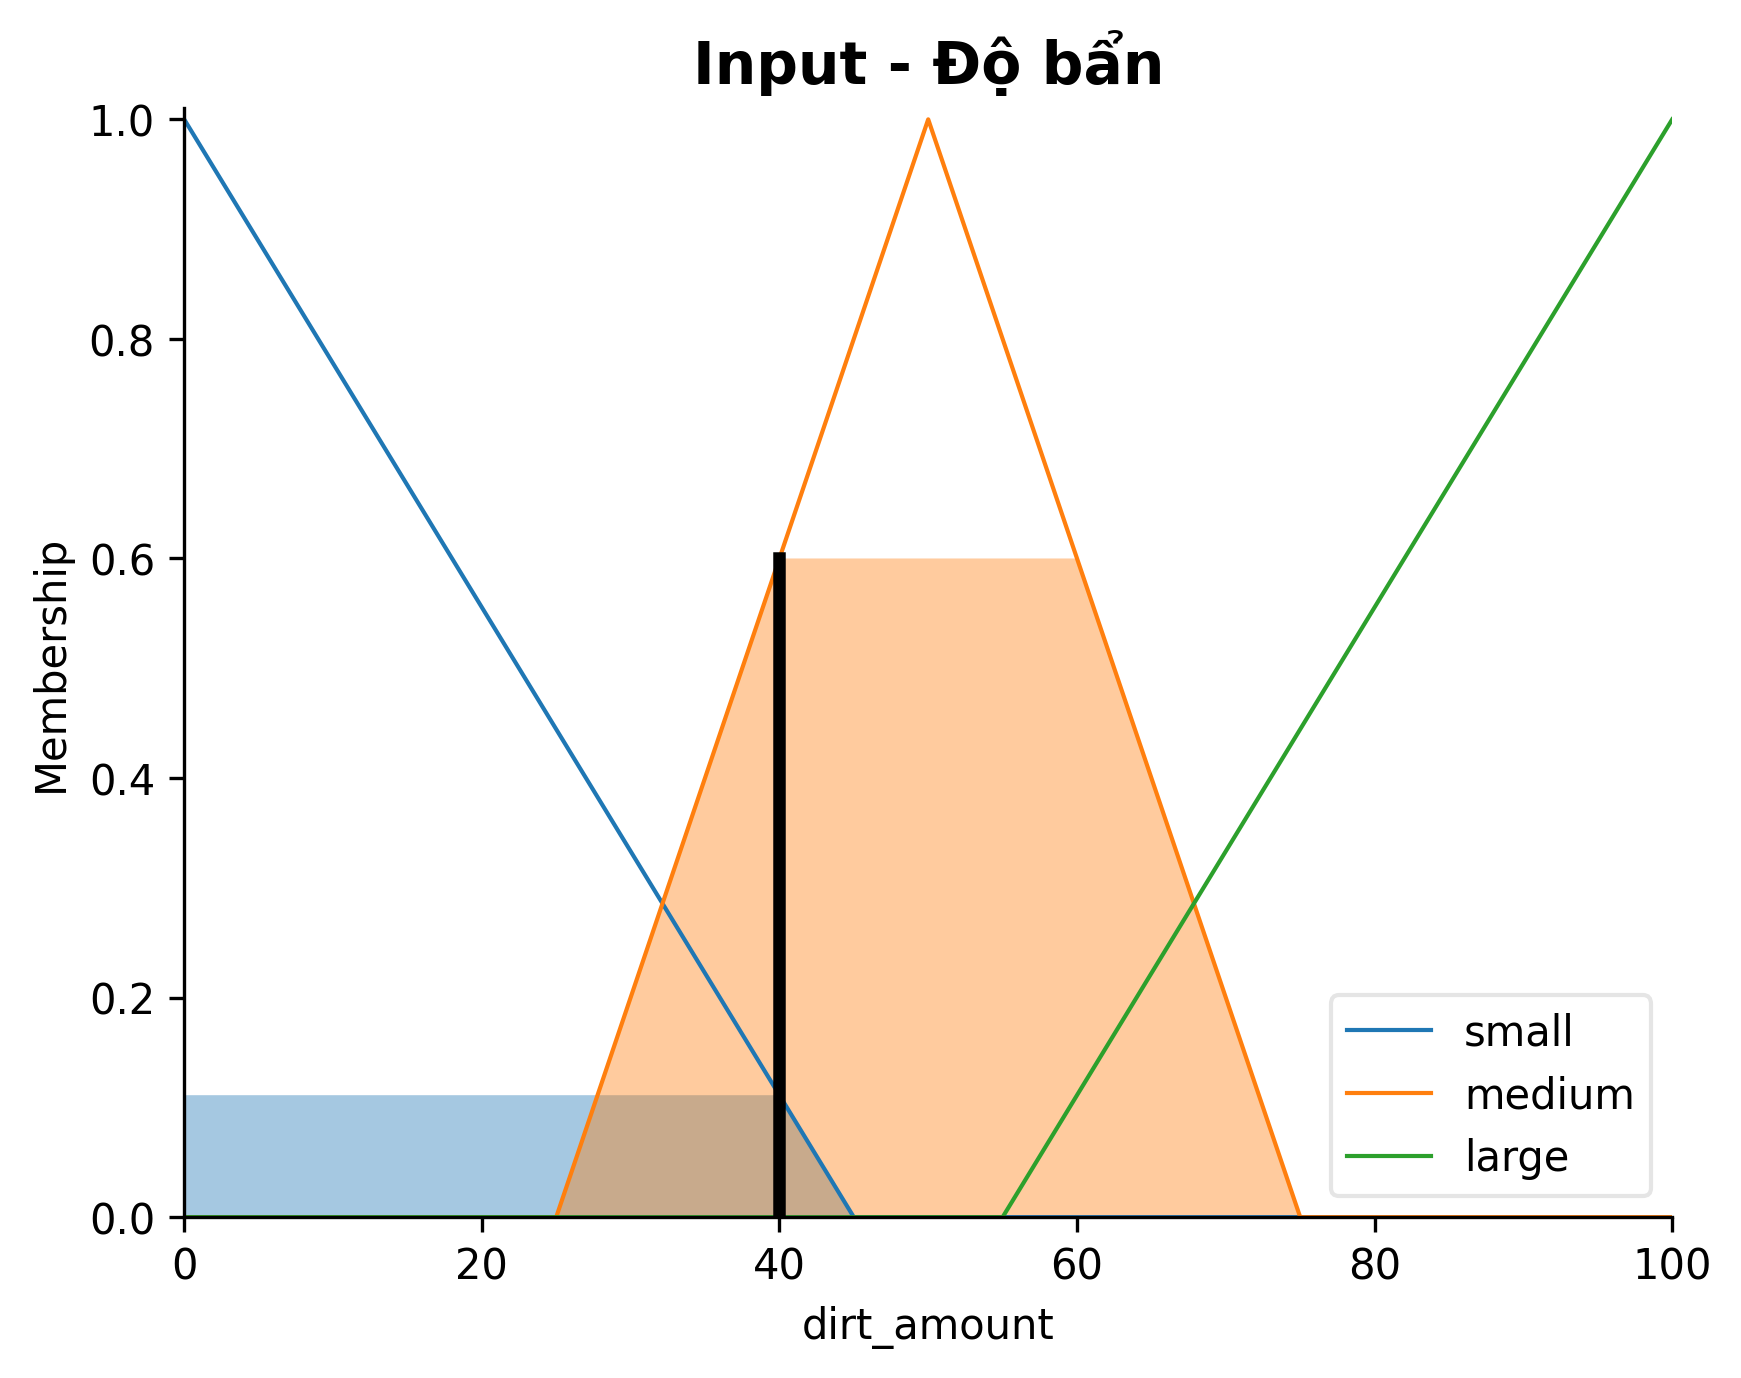
\includegraphics[width=0.7\textwidth]{images/input_dirt_amount.png}
    \caption{Đồ thị hàm liên thuộc của biến Độ bẩn}
    \label{fig:dirt_amount}
\end{figure}

\subsubsection{Mức dầu mỡ/ Loại bẩn}
\textbf{Ý nghĩa thực tiễn:} Định lượng tỷ lệ các vết bẩn cứng đầu, có cấu trúc phân tử phức tạp khó bị bẻ gãy bằng nước lạnh (như dầu mỡ công nghiệp, vết thức ăn). \\
\textbf{Không gian nền:} $X \in [0, 100]\%$.
\begin{itemize}
    \item \textbf{Tập \textit{Không dầu mỡ}:} Tọa độ $[0, 0, 45]$.
    \item \textbf{Tập \textit{Hỗn hợp}:} Tọa độ $[25, 50, 75]$.
    \item \textbf{Tập \textit{Nhiều dầu mỡ}:} Tọa độ $[55, 100, 100]$.
\end{itemize}
\textbf{Cơ chế hoạt động:} Mức độ dầu mỡ được hệ thống đánh giá gián tiếp thông qua sự thay đổi độ đục của nước sau khi kết hợp với bọt xà phòng ở những phút đầu tiên, cũng như dựa trên sức căng bề mặt của nước đo được. \\
\textbf{Biện luận thiết kế:} Ngưỡng kích hoạt $55\%$ của tập \textit{Nhiều dầu mỡ} đóng vai trò là điểm bùng phát chuyên biệt để hệ thống phát lệnh cấp điện cho thanh gia nhiệt đun nóng nước.

\begin{figure}[H]
    \centering
    
\includegraphics[width=0.7\textwidth]{images/input_dirt_type.png}
    \caption{Đồ thị hàm liên thuộc của biến Mức dầu mỡ}
    \label{fig:dirt_type}
\end{figure}

\subsubsection{Độ nhạy cảm vải}
\textbf{Ý nghĩa thực tiễn:} Đánh giá độ bền cơ học của sợi vải, khả năng chịu lực ly tâm và lực xoắn vặn. Điểm càng cao chứng tỏ sợi vải càng mỏng manh, dễ đứt gãy. \\
\textbf{Không gian nền:} $X \in [0, 10]$ điểm.
\begin{itemize}
    \item \textbf{Tập \textit{Ít nhạy cảm}:} Tọa độ $[0, 0, 4]$.
    \item \textbf{Tập \textit{Bình thường}:} Tọa độ $[2, 5, 8]$.
    \item \textbf{Tập \textit{Rất nhạy cảm}:} Tọa độ $[6, 10, 10]$.
\end{itemize}
\textbf{Cơ chế hoạt động:} Khi lồng giặt quay thử nghiệm ở pha đầu, bộ cảm biến từ trường trên động cơ truyền động trực tiếp sẽ đo lường lực dội ngược lại từ quần áo. Vải mềm sẽ rơi êm hơn vải thô cứng, từ đó trí tuệ nhân tạo sẽ chấm điểm mức độ nhạy cảm của mẻ giặt. \\
\textbf{Biện luận thiết kế:} Vùng \textit{Rất nhạy cảm} được thiết kế đặc biệt hẹp (từ điểm 6 trở lên). Khi hệ thống ghi nhận giá trị rơi vào vùng báo động này, chuỗi luật ghi đè an toàn sẽ lập tức kích hoạt nhằm khóa ngưỡng tốc độ vắt.

\begin{figure}[H]
    \centering
    
\includegraphics[width=0.7\textwidth]{images/input_cloth_sensitivity.png}
    \caption{Đồ thị hàm liên thuộc của biến Độ nhạy cảm vải}
    \label{fig:cloth_sensitivity}
\end{figure}

% ---------------------------------------------------------
\subsection{Định nghĩa không gian và tham số biến đầu ra (Outputs)}
Khác với cảm biến thu thập dữ liệu đầu vào, các biến đầu ra là những tín hiệu ra lệnh trực tiếp đến các bộ phận của máy giặt, quyết định hiệu năng làm sạch và tuổi thọ thiết bị.

\subsubsection{Thời gian giặt}
\textbf{Ý nghĩa thực tiễn:} Tổng thời lượng duy trì nhịp độ nhào lộn của lồng giặt nhằm đánh bật vết bẩn trước khi xả nước. \\
\textbf{Không gian nền:} $Y \in [0, 180]$ phút. 
\begin{itemize}
    \item \textbf{Tập \textit{Rất ngắn}:} Tọa độ $[0, 20, 45]$.
    \item \textbf{Tập \textit{Ngắn}:} Tọa độ $[25, 50, 75]$.
    \item \textbf{Tập \textit{Vừa}:} Tọa độ $[55, 80, 105]$.
    \item \textbf{Tập \textit{Dài}:} Tọa độ $[85, 110, 135]$.
    \item \textbf{Tập \textit{Rất dài}:} Tọa độ $[115, 150, 180]$.
\end{itemize}
\textbf{Cơ chế hoạt động:} Vi điều khiển nhận giá trị thời gian cụ thể vừa được giải mờ và nạp trực tiếp vào bộ đếm thời gian của máy giặt. Con số này thiết lập tổng thời lượng duy trì chu kỳ đảo chiều động cơ trước khi chuyển sang pha xả nước. \\
\textbf{Biện luận thiết kế:} Việc phân bổ thành 5 dải thời gian với khoảng giao thoa hợp lý giúp hệ thống tránh được tình trạng thời gian giặt bị nhảy vọt đột ngột khi khối lượng quần áo chỉ tăng thêm vài trăm gram, tối ưu hóa trải nghiệm người dùng.

\begin{figure}[H]
    \centering
    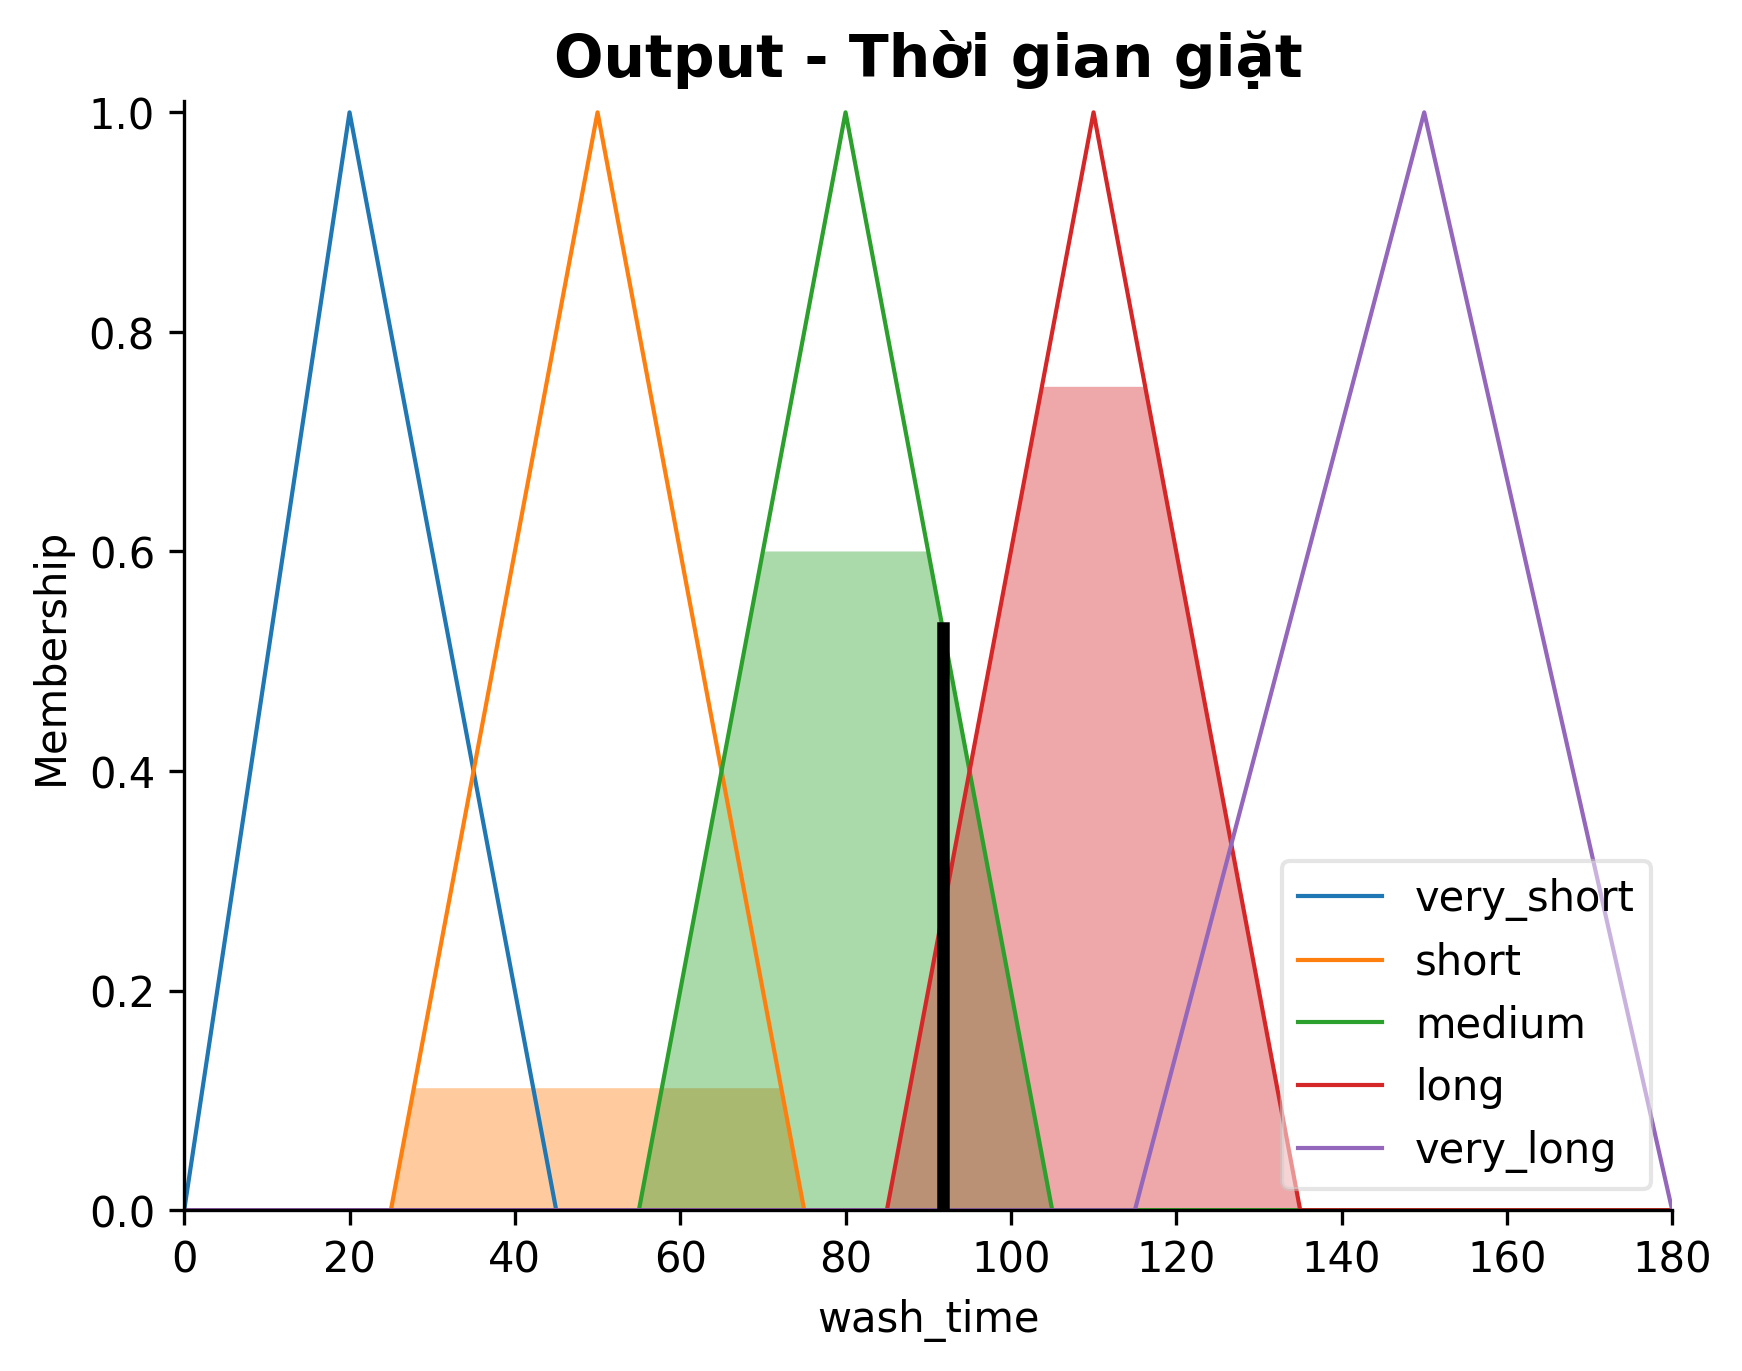
\includegraphics[width=0.7\textwidth]{images/output_wash_time.png}
    \caption{Đồ thị hàm liên thuộc của biến đầu ra Thời gian giặt}
    \label{fig:wash_time}
\end{figure}

\subsubsection{Tốc độ vắt}
\textbf{Ý nghĩa thực tiễn:} Tốc độ vòng quay tối đa của lồng giặt ở pha cuối cùng nhằm tạo ra lực ly tâm ép kiệt nước ra khỏi sợi vải. \\
\textbf{Không gian nền:} $Y \in [0, 1400]$ vòng/phút (RPM).
\begin{itemize}
    \item \textbf{Tập \textit{Rất thấp}:} Tọa độ $[0, 300, 550]$.
    \item \textbf{Tập \textit{Thấp}:} Tọa độ $[400, 650, 850]$.
    \item \textbf{Tập \textit{Vừa}:} Tọa độ $[700, 900, 1050]$.
    \item \textbf{Tập \textit{Cao}:} Tọa độ $[900, 1100, 1250]$.
    \item \textbf{Tập \textit{Rất cao}:} Tọa độ $[1150, 1350, 1400]$.
\end{itemize}
\textbf{Cơ chế hoạt động:} Lệnh điều khiển được truyền xuống bo mạch biến tần để điều tiết dòng điện cấp cho động cơ chính. Hệ thống logic mờ cho phép lồng giặt tăng tốc cực kỳ êm ái và bám sát vào đúng số vòng quay lẻ đã được tính toán (ví dụ: 883 vòng/phút), triệt tiêu hoàn toàn sự rung lắc do thay đổi gia tốc đột ngột. \\
\textbf{Biện luận thiết kế:} Các dải vận tốc cao được thiết kế có độ dốc lớn để thuật toán dễ dàng cắt ngọn và hãm phanh tức thời khi phát hiện có quần áo bằng lụa mỏng dệt đan xen.

\begin{figure}[H]
    \centering
    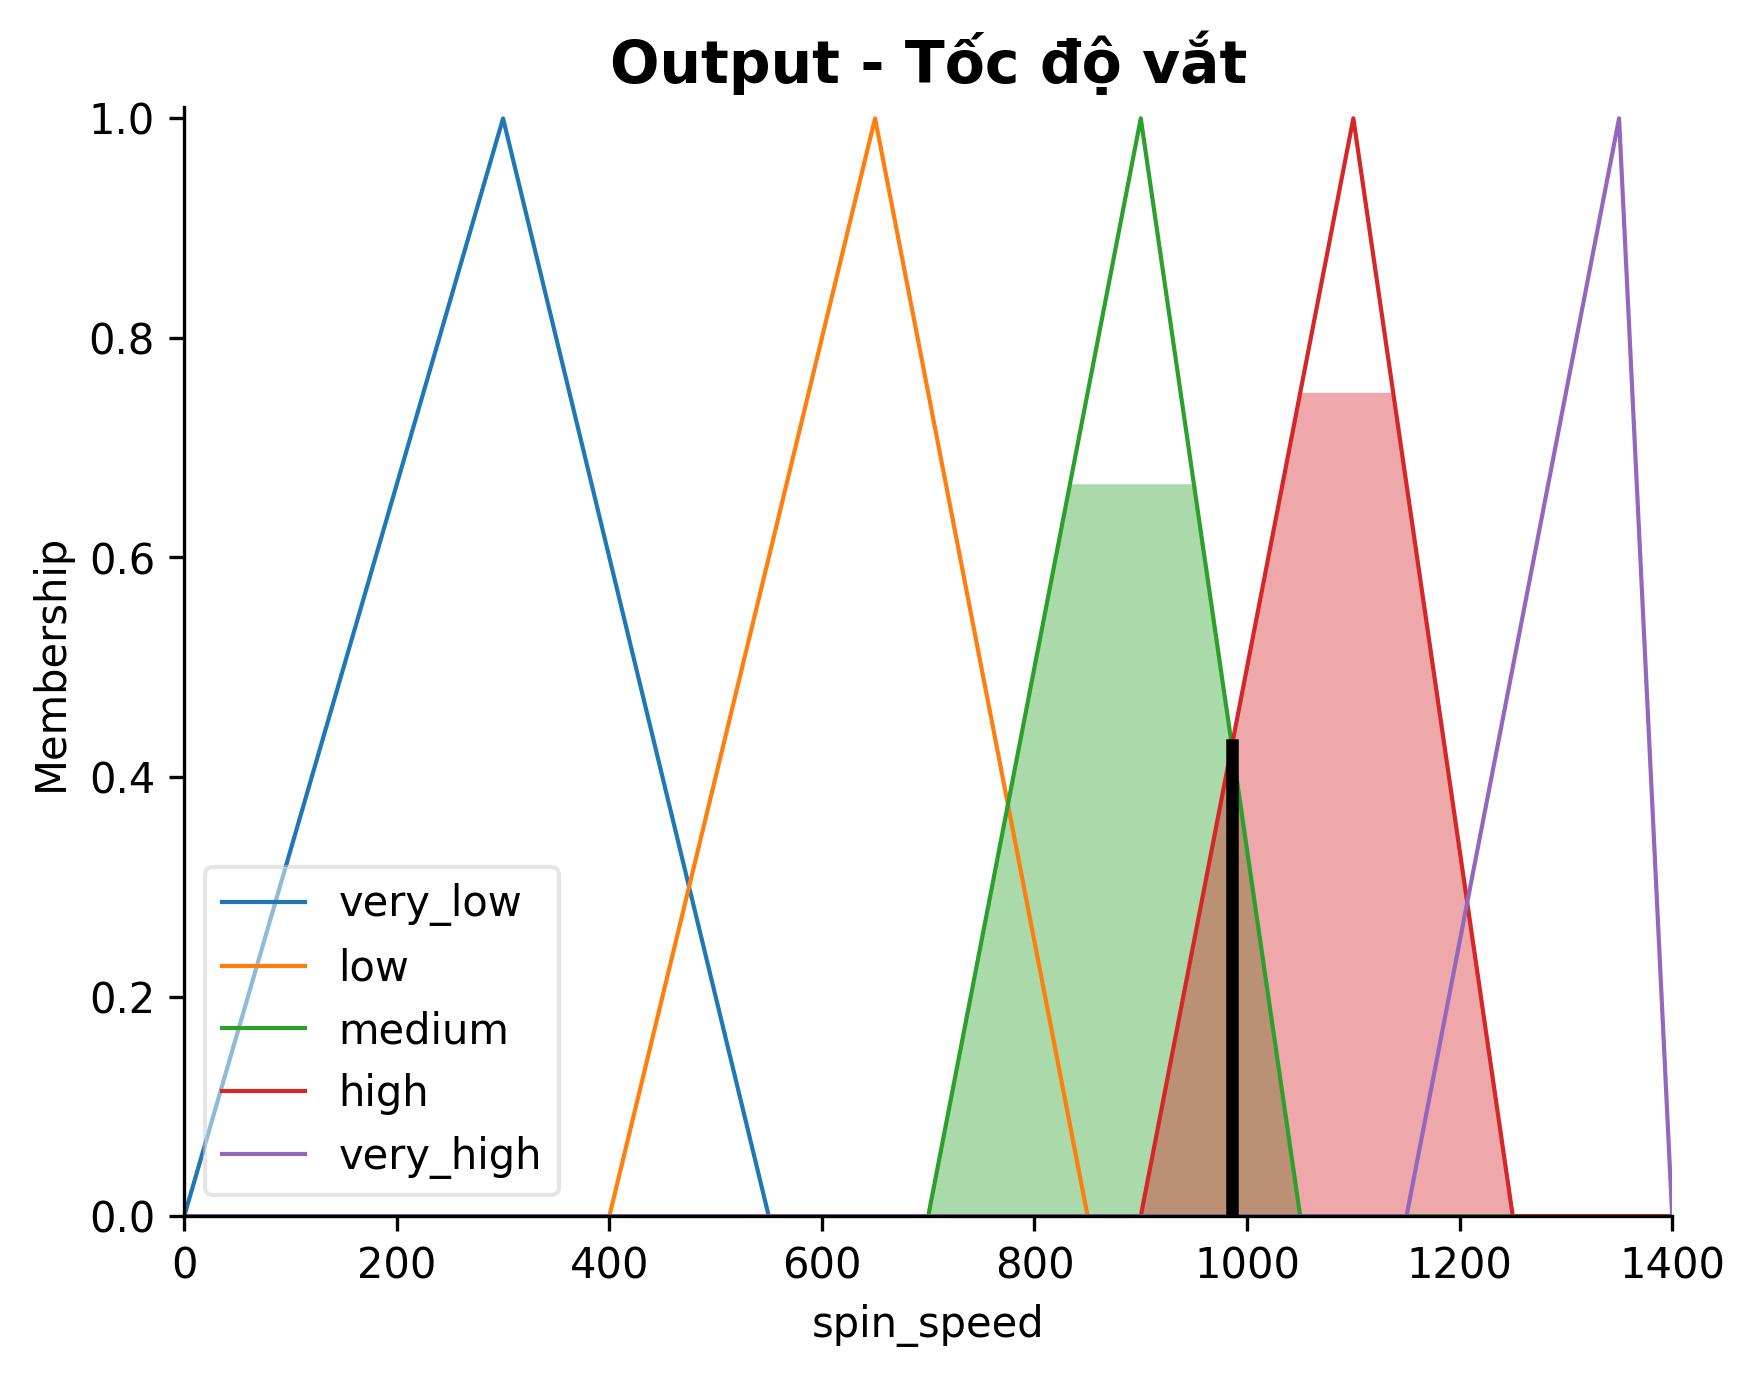
\includegraphics[width=0.7\textwidth]{images/output_spin_speed.png}
    \caption{Đồ thị hàm liên thuộc của biến đầu ra Tốc độ vắt}
    \label{fig:spin_speed}
\end{figure}

\subsubsection{Lượng nước}
\textbf{Ý nghĩa thực tiễn:} Thể tích nước tối ưu cần cấp vào lồng giặt để hòa tan xà phòng và tạo không gian nhào lộn êm ái cho quần áo. \\
\textbf{Không gian nền:} $Y \in [0, 100]\%$.
\begin{itemize}
    \item \textbf{Tập \textit{Ít}:} Tọa độ $[0, 0, 40]$.
    \item \textbf{Tập \textit{Bình thường}:} Tọa độ $[20, 50, 80]$.
    \item \textbf{Tập \textit{Nhiều}:} Tọa độ $[60, 100, 100]$.
\end{itemize}
\textbf{Cơ chế hoạt động:} Giá trị phần trăm (\%) xuất ra từ thuật toán sẽ quyết định thời gian mở của van cấp nước tự động. Đồng thời, phao cảm biến áp suất bên trong lồng giặt sẽ liên tục đo lường mực nước thực tế và phản hồi về hệ thống để ngắt van điện từ ngay khi đạt chuẩn. \\
\textbf{Biện luận thiết kế:} Việc đặt đỉnh của tập mờ \textit{Bình thường} nằm đúng ở chính giữa thang đo ($50\%$) tạo ra cấu trúc đối xứng, giúp thuật toán luôn có xu hướng cân bằng lượng nước cấp vào, tránh xả ngập nước dư thừa gây lãng phí sinh thái.

\begin{figure}[H]
    \centering
    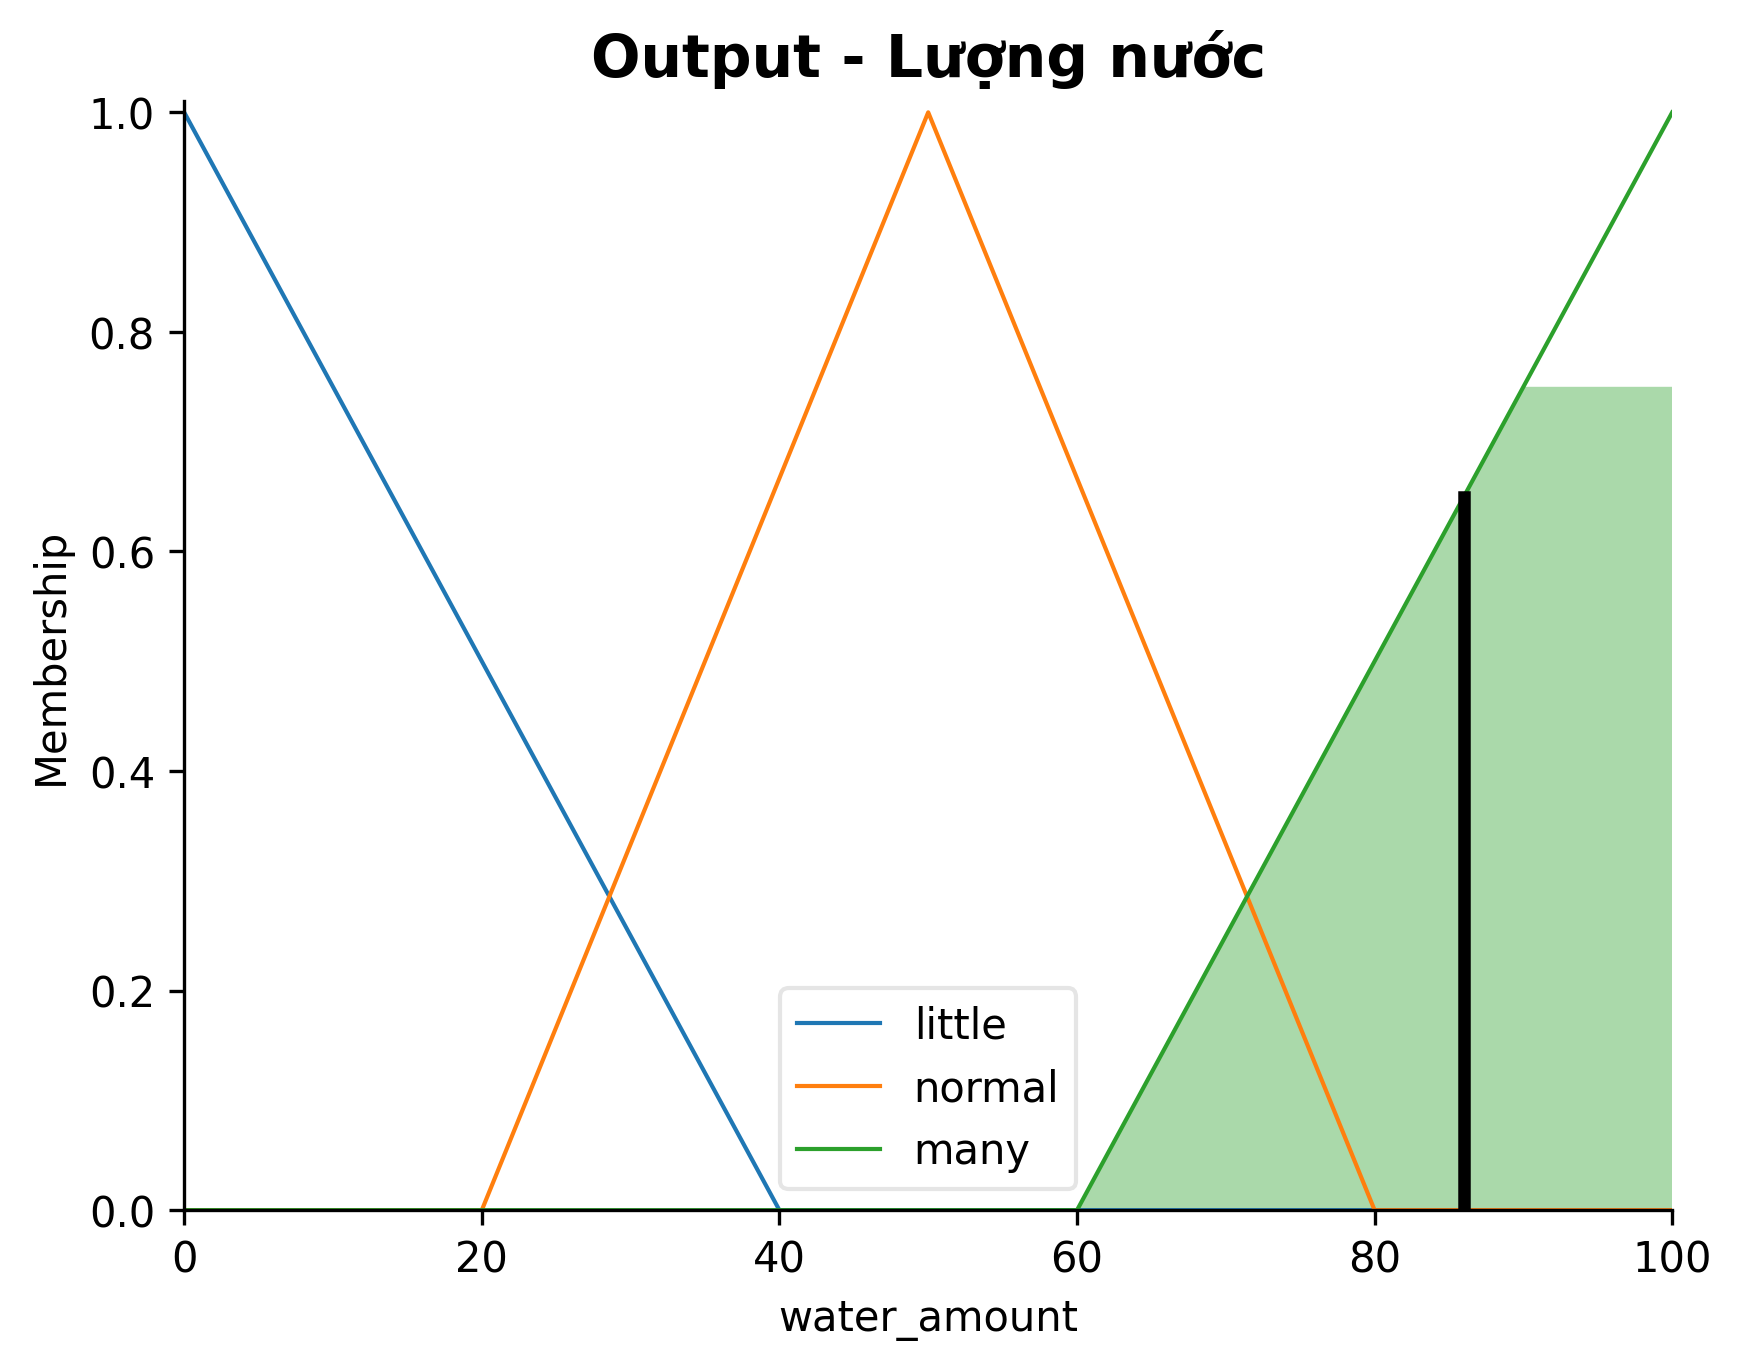
\includegraphics[width=0.7\textwidth]{images/output_water_amount.png}
    \caption{Đồ thị hàm liên thuộc của biến đầu ra Lượng nước}
    \label{fig:water_amount}
\end{figure}

\subsubsection{Lượng xà phòng}
\textbf{Ý nghĩa thực tiễn:} Tỷ lệ hóa chất tẩy rửa cần thiết để bẻ gãy các liên kết chất bẩn mà không để lại cặn tồn dư trên quần áo. \\
\textbf{Không gian nền:} $Y \in [0, 100]\%$.
\begin{itemize}
    \item \textbf{Tập \textit{Ít}:} Tọa độ $[0, 0, 40]$.
    \item \textbf{Tập \textit{Bình thường}:} Tọa độ $[20, 50, 80]$.
    \item \textbf{Tập \textit{Nhiều}:} Tọa độ $[60, 100, 100]$.
\end{itemize}
\textbf{Cơ chế hoạt động:} Lệnh điều khiển tác động trực tiếp lên hệ thống chiết rót thông minh của ngăn chứa nước giặt. Bơm điện sẽ tự động hút chính xác một thể tích xà phòng tương ứng với tỷ lệ phần trăm đã nội suy và hòa tan ngay vào dòng nước cấp. Cơ chế này loại bỏ hoàn toàn thói quen đổ xà phòng theo cảm tính của người dùng. \\
\textbf{Biện luận thiết kế:} Sự đồng bộ tuyệt đối về cấu trúc tọa độ giữa biến Lượng nước và biến Xà phòng giúp bộ điều khiển luôn thiết lập được một tỷ lệ hòa tan hóa chất chuẩn xác nhất ở mọi kịch bản.

\begin{figure}[H]
    \centering
    
\includegraphics[width=0.7\textwidth]{images/output_detergent.png}
    \caption{Đồ thị hàm liên thuộc của biến đầu ra Lượng xà phòng}
    \label{fig:detergent}
\end{figure}

\subsubsection{Nhiệt độ nước}
\textbf{Ý nghĩa thực tiễn:} Mức nhiệt năng cần thiết để xúc tác cho các phản ứng hóa học của xà phòng, cực kỳ quan trọng trong việc làm tan rã dầu mỡ. \\
\textbf{Không gian nền:} $Y \in [0, 100]^\circ\text{C}$.
\begin{itemize}
    \item \textbf{Tập \textit{Thấp}:} Tọa độ $[0, 20, 45]$.
    \item \textbf{Tập \textit{Vừa}:} Tọa độ $[30, 45, 65]$.
    \item \textbf{Tập \textit{Cao}:} Tọa độ $[55, 95, 100]$.
\end{itemize}
\textbf{Cơ chế hoạt động:} Dựa trên kết quả giải mờ, bo mạch chủ sẽ quyết định có đóng công tắc cấp điện cho thanh điện trở gia nhiệt nằm dưới đáy lồng giặt hay không. Ngay khi nước bắt đầu ấm lên, cảm biến nhiệt độ sẽ liên tục đo đạc để hệ thống chủ động ngắt điện ngay khi nước đạt đúng ngưỡng yêu cầu (ví dụ: $46^\circ$C). \\
\textbf{Biện luận thiết kế:} Vì việc đun nóng nước tiêu tốn lượng điện năng cực kỳ lớn, thuật toán được lập trình rất khắt khe. Tập mờ \textit{Cao} chỉ cho phép kích hoạt khi hệ thống thực sự phát hiện thấy tỷ lệ vết bẩn cứng đầu vượt mức cho phép.

\begin{figure}[H]
    \centering
    
\includegraphics[width=0.7\textwidth]{images/output_water_temp.png}
    \caption{Đồ thị hàm liên thuộc của biến đầu ra Nhiệt độ nước}
    \label{fig:water_temp}
\end{figure}

% ---------------------------------------------------------
\subsection{Tập luật mờ}
\subsubsection{Bài toán không gian tổ hợp và Kỹ thuật tối ưu hóa tập luật}
Sau khi hoàn thiện việc không gian hóa các biến ngôn ngữ, bước mang tính quyết định tiếp theo là xây dựng cơ sở tri thức cho bộ điều khiển. Về mặt toán học, hệ thống có 4 biến đầu vào, mỗi biến được chia làm 3 tập mờ. Nếu thực hiện tổ hợp chập toàn bộ không gian trạng thái, tổng số quy luật mờ có thể sinh ra là $3 \times 3 \times 3 \times 3 = 81$ quy luật.

Tuy nhiên, dưới góc độ của thiết kế thuật toán ứng dụng, việc nạp toàn bộ 81 luật vào bộ nhớ của vi điều khiển sẽ gây ra hiện tượng dư thừa dữ liệu và làm tăng đáng kể độ trễ tính toán. Hơn nữa, trong thực tế sẽ có những tổ hợp điều kiện mang tính mâu thuẫn logic, ví dụ như quần áo rất bẩn và nhiều dầu mỡ nhưng lại được yêu cầu giặt cực nhanh. Do đó, nhóm nghiên cứu đã tiến hành kỹ thuật cắt tỉa luật dựa trên hệ chuyên gia của dòng máy LG AI DD. Kết quả là không gian 81 luật đã được tối ưu hóa và cô đọng lại thành một ma trận gồm 19 quy luật mờ cốt lõi dạng mệnh đề NẾU-THÌ. Sự tinh giản này vừa đảm bảo phủ kín các trường hợp vận hành thực tế, vừa tối ưu hóa chu kỳ quét của toàn hệ thống.

\subsubsection{Cấu trúc và Phân tầng hệ thống luật mờ}
Hệ thống sử dụng cơ chế suy diễn Mamdani, trong đó mệnh đề điều kiện của các luật sử dụng toán tử logic VÀ, được thực thi bằng phép toán \textit{t-norm} lấy giá trị cực tiểu, để liên kết các biến đầu vào. Từ đó, hệ thống nội suy ra tổ hợp 5 lệnh đầu ra ở mệnh đề kết luận. Để đảm bảo tính chặt chẽ, ma trận 19 quy luật mờ này được phân tầng logic thành ba lớp chuyên biệt như sau:

\begin{itemize}
    \item \textbf{Lớp thứ nhất - Nhóm luật kịch bản toàn diện:} Đây là bộ khung xương sống của hệ thống, bao gồm các luật vĩ mô đánh giá đồng thời cả 4 thông số đầu vào để nội suy ra một chu trình giặt hoàn chỉnh. Ví dụ với Luật số 1 áp dụng cho kịch bản tải nặng và đồ bảo hộ lao động: NẾU khối lượng ở mức Nhiều, độ bẩn Nhiều, dầu mỡ Nhiều và độ nhạy cảm của vải ở mức Ít, THÌ hệ thống sẽ xuất ra chuỗi lệnh điều khiển đạt ngưỡng tối đa bao gồm thời gian giặt Rất dài, tốc độ vắt Rất cao và nhiệt độ nước Cao. Nhóm luật này giúp máy giặt định hình chế độ vận hành cơ sở một cách nhanh chóng nhất.
    
    \item \textbf{Lớp thứ hai - Nhóm luật bổ trợ và tối ưu tài nguyên:} Thay vì can thiệp vào toàn bộ 5 biến đầu ra, nhóm luật này hoạt động ở mức vi mô, chỉ tinh chỉnh một vài thông số nhất định nhằm tối ưu hóa năng lượng sinh thái. Lấy ví dụ với Luật số 7 và Luật số 8 về tối ưu hóa lượng nước và xà phòng: Dựa trên tín hiệu trọng lượng lồng giặt, hệ thống thiết lập quy tắc tự động gia giảm lượng nước và xà phòng tỷ lệ thuận với khối lượng quần áo. Sự can thiệp độc lập này giúp giải quyết bài toán lãng phí tài nguyên của các thế hệ máy giặt lồng ngang đời cũ mà không làm phá vỡ cấu trúc thời gian của mẻ giặt.
    
    \item \textbf{Lớp thứ ba - Nhóm luật ghi đè an toàn:} Đây là điểm nhấn đột phá và mang lại giá trị thực tiễn cao nhất cho hệ thống. Trong lĩnh vực tự động hóa, sự an toàn của đối tượng bị tác động (quần áo) phải được đặt lên hàng đầu. Nhóm luật này được cấp quyền ưu tiên cao nhất, cho phép vượt quyền các điều kiện thông thường để ép buộc hệ thống thực thi lệnh bảo vệ. Ví dụ điển hình là Luật số 9 nhằm bảo vệ đồ lụa hoặc vải mỏng: Bất chấp việc quần áo có mức độ bẩn hay khối lượng lớn đến đâu, chỉ cần cảm biến đánh giá thông số độ nhạy cảm của vải ở mức Rất nhạy cảm, hệ thống sẽ lập tức kích hoạt luật an toàn để khóa cứng vòng vắt ở mức Thấp hoặc Rất thấp. Sự ghi đè này triệt tiêu hoàn toàn rủi ro xé rách sợi vải do lực ly tâm sinh ra ở tốc độ vòng quay lớn. Tương tự, một số luật an toàn khác sẽ ép buộc mở rơ-le nhiệt độ Cao ngay khi phát hiện tỷ lệ vết bẩn cứng đầu vượt ngưỡng cho phép.
\end{itemize}

Sự tương tác, bù trừ và chồng chập của ba lớp luật này trong không gian hình học đa chiều đã tạo ra các mặt cong điều khiển vô cùng mượt mà. Một số luật tiêu biểu mang tính đại diện cho ma trận 19 quy luật trên được trích xuất và trình bày chi tiết trong bảng tổng hợp dưới đây:

\begin{table}[H]
    \centering
    \caption{Trích xuất các luật mờ cốt lõi của hệ thống}
    \label{tab:fuzzy_rules}
    \resizebox{\textwidth}{!}{
    \renewcommand{\arraystretch}{1.5}
    \begin{tabular}{|c|p{3cm}|p{6.5cm}|p{6cm}|}
        \hline
        \textbf{Phân lớp} & \textbf{Luật tiêu biểu} & \textbf{Mệnh đề Điều kiện (IF)} & \textbf{Mệnh đề Kết luận (THEN)} \\
        \hline
        \multirow{2}{*}{Lớp 1} & Rule 1: Tải nặng & Khối lượng (\textit{Nhiều}) AND Độ bẩn (\textit{Nhiều}) AND Dầu mỡ (\textit{Nhiều}) AND Vải (\textit{Ít nhạy cảm}) & Thời gian (\textit{Rất dài}), Vắt (\textit{Rất cao}), Nước (\textit{Nhiều}), Xà phòng (\textit{Nhiều}), Nhiệt độ (\textit{Cao}) \\ \cline{2-4}
        & Rule 2: Bảo vệ vải & Khối lượng (\textit{Ít}) AND Độ bẩn (\textit{Ít}) AND Dầu mỡ (\textit{Ít}) AND Vải (\textit{Rất nhạy cảm}) & Thời gian (\textit{Rất ngắn}), Vắt (\textit{Rất thấp}), Nước (\textit{Ít}), Xà phòng (\textit{Ít}), Nhiệt độ (\textit{Thấp}) \\
        \hline
        Lớp 2 & Rule 7/8: Tiết kiệm & Tải trọng (\textit{Ít} hoặc \textit{Nhiều}) & Tự động gia giảm cấu hình Lượng nước và Xà phòng tương ứng. \\
        \hline
        Lớp 3 & Rule 9: Ghi đè & Nhạy cảm vải (\textit{Rất nhạy cảm}) hoặc Dầu mỡ (\textit{Nhiều}) & Ép buộc khóa tốc độ vắt ở mức (\textit{Thấp}) hoặc kích hoạt nhiệt độ (\textit{Cao}) vô điều kiện. \\
        \hline
    \end{tabular}
    }
\end{table}

% ===================================================================
% CHƯƠNG 4: CÀI ĐẶT VÀ MÔ PHỎNG
% ===================================================================
\section{Cài đặt và Mô phỏng}

\subsection{Môi trường và thư viện phát triển}
Hệ thống được lập trình trên môi trường Python 3.11. Thư viện cốt lõi là \textbf{scikit-fuzzy} \cite{skfuzzy}, đảm nhiệm toàn bộ engine suy diễn Mamdani, từ mờ hóa đến giải mờ tích phân rời rạc (COA). 

Dưới đây là một đoạn \textit{snippet code} minh họa cách nhóm khởi tạo không gian nền, định nghĩa hàm liên thuộc và thiết lập luật mờ thông qua các hàm API của thư viện:

\begin{lstlisting}[caption={Minh họa cách định nghĩa biến và luật mờ bằng skfuzzy}, label={lst:fuzzy_snippet}]
import skfuzzy.control as ctrl
import skfuzzy as fuzz
import numpy as np

# 1. Khoi tao khong gian nen (Universe)
cloth_amount = ctrl.Antecedent(np.arange(0, 10.5, 0.5), 'cloth_amount')
dirt_amount = ctrl.Antecedent(np.arange(0, 101, 1), 'dirt_amount')
spin_speed = ctrl.Consequent(np.arange(0, 1401, 1), 'spin_speed')

# 2. Dinh nghia toa do ham lien thuoc (Trimf)
cloth_amount['Nhieu'] = fuzz.trimf(cloth_amount.universe, [6, 10, 10])
dirt_amount['Rat_ban'] = fuzz.trimf(dirt_amount.universe, [55, 100, 100])
spin_speed['Rat_cao'] = fuzz.trimf(spin_speed.universe, [1050, 1400, 1400])

# 3. Khai bao luat mo (Menh de IF-THEN)
rule_1 = ctrl.Rule(
    cloth_amount['Nhieu'] & dirt_amount['Rat_ban'], 
    spin_speed['Rat_cao']
)
\end{lstlisting}

Các thư viện hỗ trợ bao gồm \textbf{NumPy} để xử lý ma trận và \textbf{Streamlit, Plotly} để xây dựng kiến trúc giao diện tương tác (GUI).

\subsection{Giao diện người dùng và Trực quan hóa kết quả}
Toàn bộ giao diện được triển khai dưới dạng ứng dụng web tại địa chỉ \url{https://washai.streamlit.app/}, không yêu cầu cài đặt phía người dùng. Mỗi thay đổi trên thanh trượt đầu vào đều kích hoạt tức thời một vòng tính toán đầy đủ của engine \textit{skfuzzy} và cập nhật đồng thời tất cả các thành phần hiển thị.

\subsubsection{Cấu hình đầu vào}
Phân hệ này được bố trí tại cột trái, đóng vai trò như một bộ giả lập cảm biến. Người dùng có thể lựa chọn nhanh các kịch bản giặt hoặc can thiệp thủ công vào 4 biến đầu vào thông qua các thanh trượt. Hệ thống hỗ trợ nhập giá trị liên tục cho Độ bẩn ($0-100\%$), Mức dầu mỡ ($0-100\%$) và Khối lượng ($0-10$ kg), mô phỏng chính xác dải tín hiệu thực tế truyền về từ các cảm biến vật lý.

\begin{figure}[H]
    \centering
    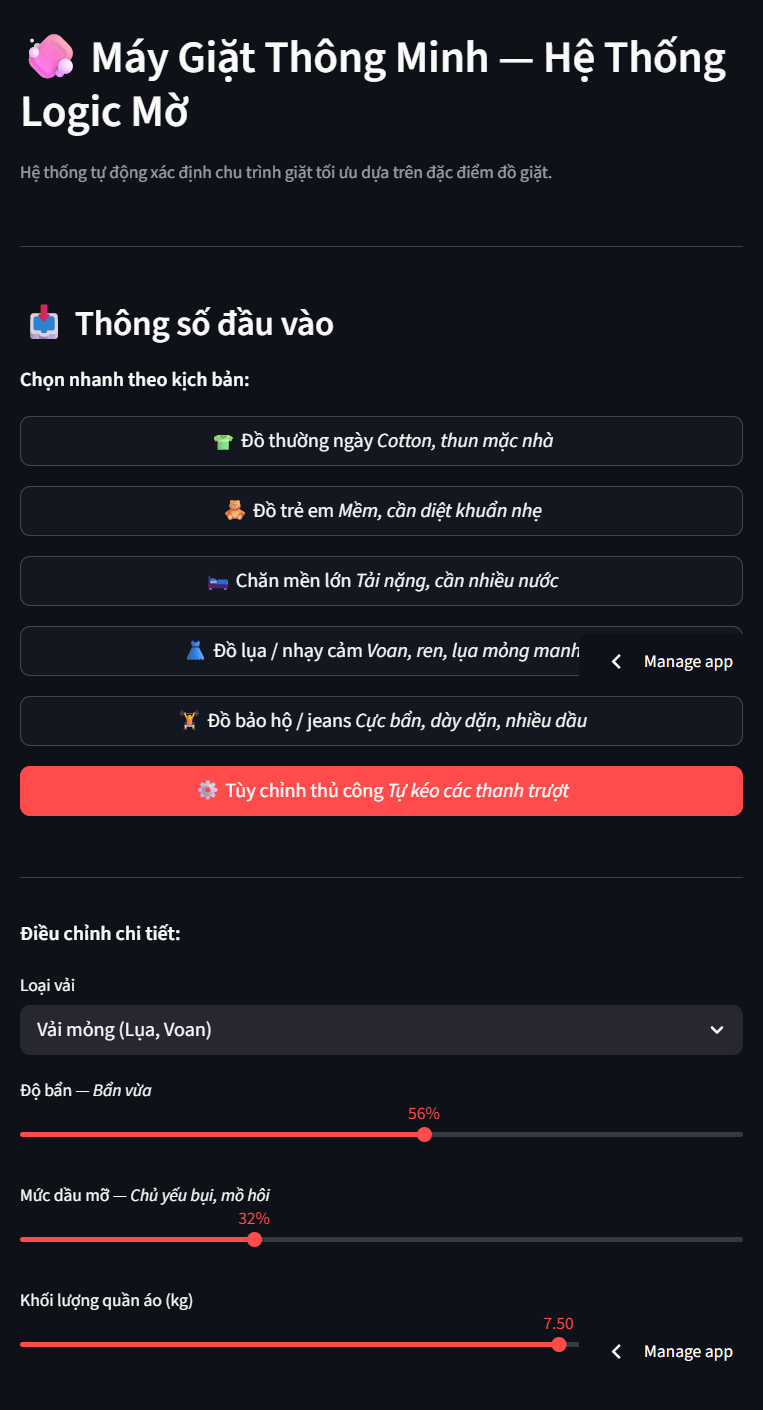
\includegraphics[width=0.65\textwidth]{images/gui.png} 
    \caption{Phân hệ giả lập thông số cảm biến đầu vào}
    \label{fig:gui}
\end{figure}

\subsubsection{Phân hệ đầu ra và các Tab phân tích chuyên môn}
Ngay khi dữ liệu đầu vào thay đổi, hệ thống thực thi engine suy diễn mờ và cập nhật các lệnh điều khiển. Các thông số này được bóc tách chi tiết qua 4 Tab chức năng:

\textbf{1. Tab Phân tích chi tiết:} \\
Cung cấp góc nhìn thực tiễn về chu trình vận hành. Tổng thời gian giặt được phân bổ thành 4 pha vận hành: Ngâm (chiếm khoảng 19\%), Giặt (chiếm khoảng 45\%), Xả (chiếm khoảng 22\%) và Vắt (chiếm khoảng 14\%), mỗi pha được hiển thị bằng thanh tiến trình riêng biệt. Cụ thể, thanh tiến trình tốc độ vắt được chia thành 5 vùng màu từ \textit{"Rất nhẹ (Lụa)"} đến \textit{"Tối đa (Jeans)"}, trong đó nhãn ngôn ngữ cập nhật động theo giá trị RPM hiện tại (ví dụ: \textit{"Trung bình — 783 RPM"}). 

\begin{figure}[H]
    \centering
    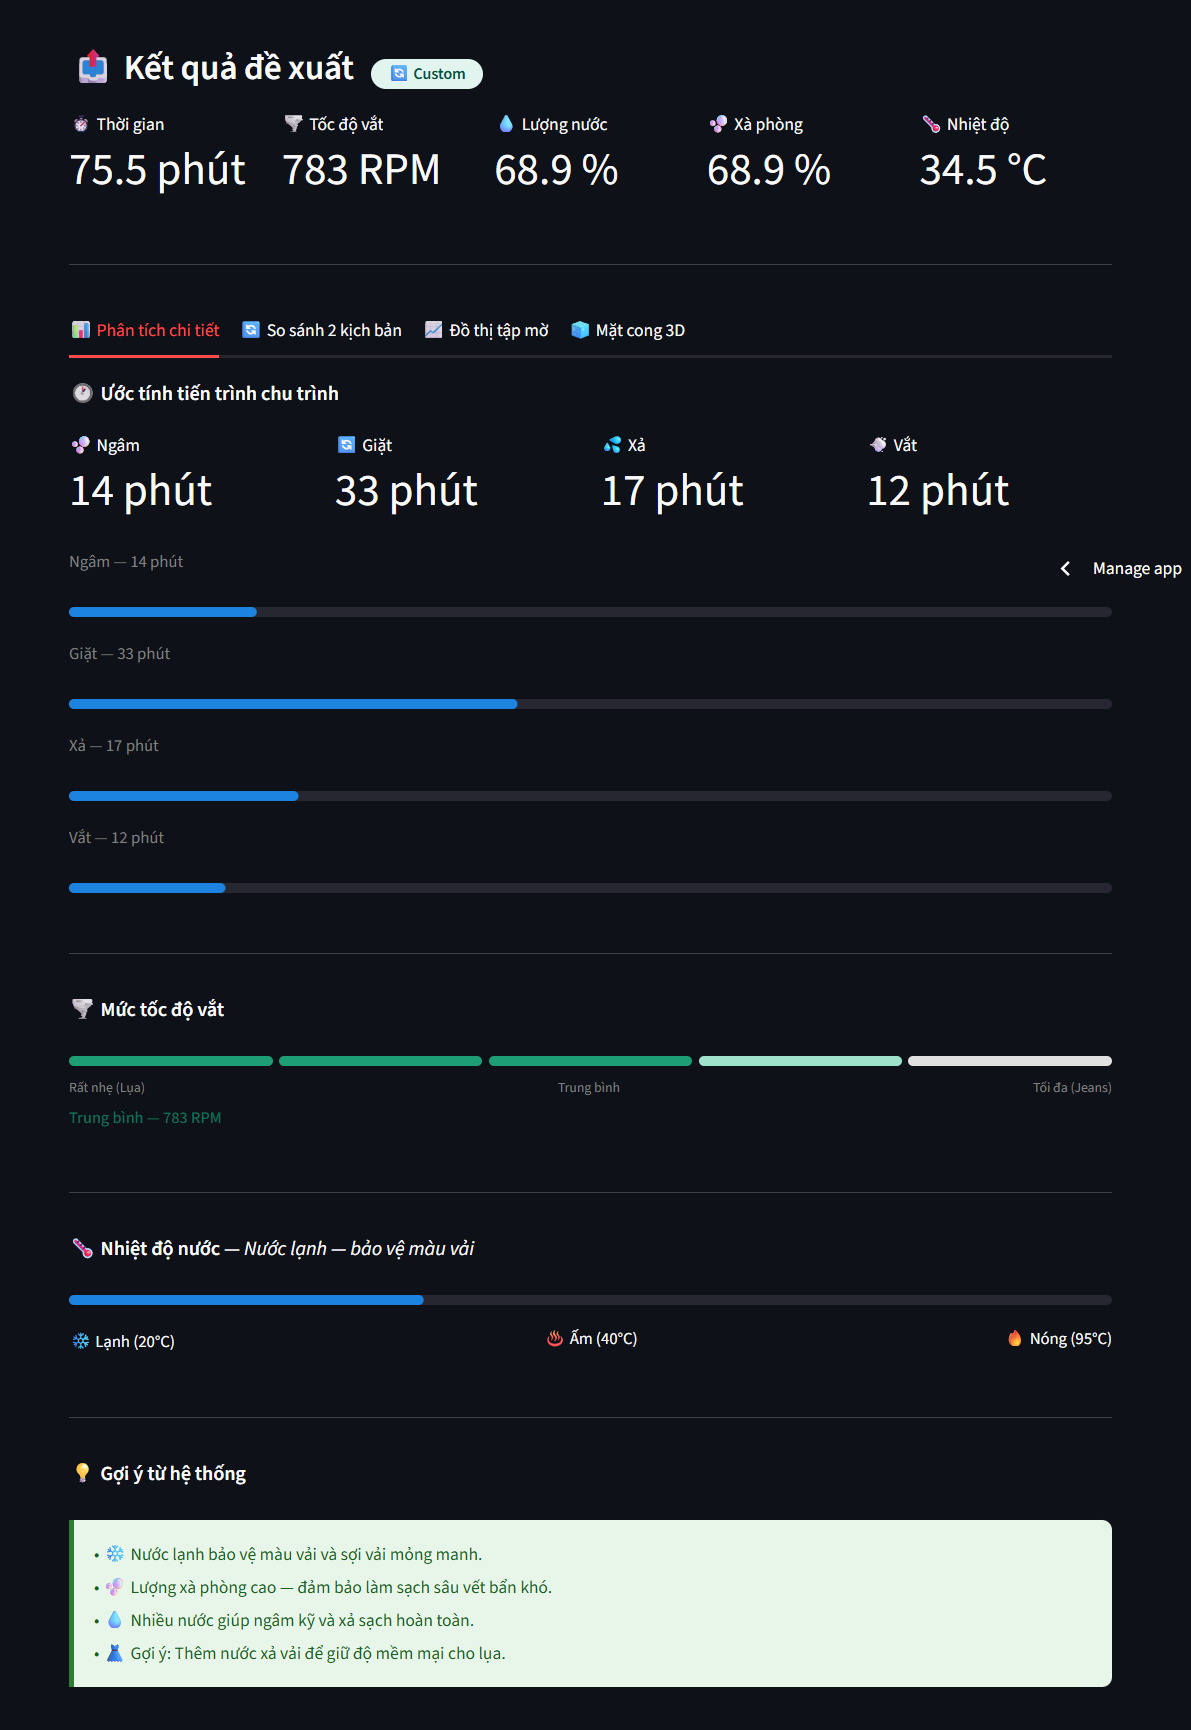
\includegraphics[width=0.9\textwidth]{images/tab_phantich.png} 
    \caption{Tab Phân tích chi tiết và khuyến nghị vận hành}
    \label{fig:tab_phantich}
\end{figure}

\textbf{2. Tab So sánh 2 kịch bản:} \\
Chức năng này cho phép chọn độc lập Kịch bản A và Kịch bản B để so sánh. Hệ thống render song song 5 cặp thanh ngang: màu xanh biểu thị Kịch bản A và màu cam biểu thị Kịch bản B. Bên cạnh giá trị tuyệt đối, hệ thống tính toán delta chênh lệch kèm chiều tăng/giảm (ví dụ: $+150.0$ RPM, $-10.9^\circ$C). Khung nhận xét cuối tab tự động tổng hợp chênh lệch thành ngôn ngữ định tính, minh chứng cho tính liên tục của Logic mờ (đáp ứng RQ3).

\begin{figure}[H]
    \centering
    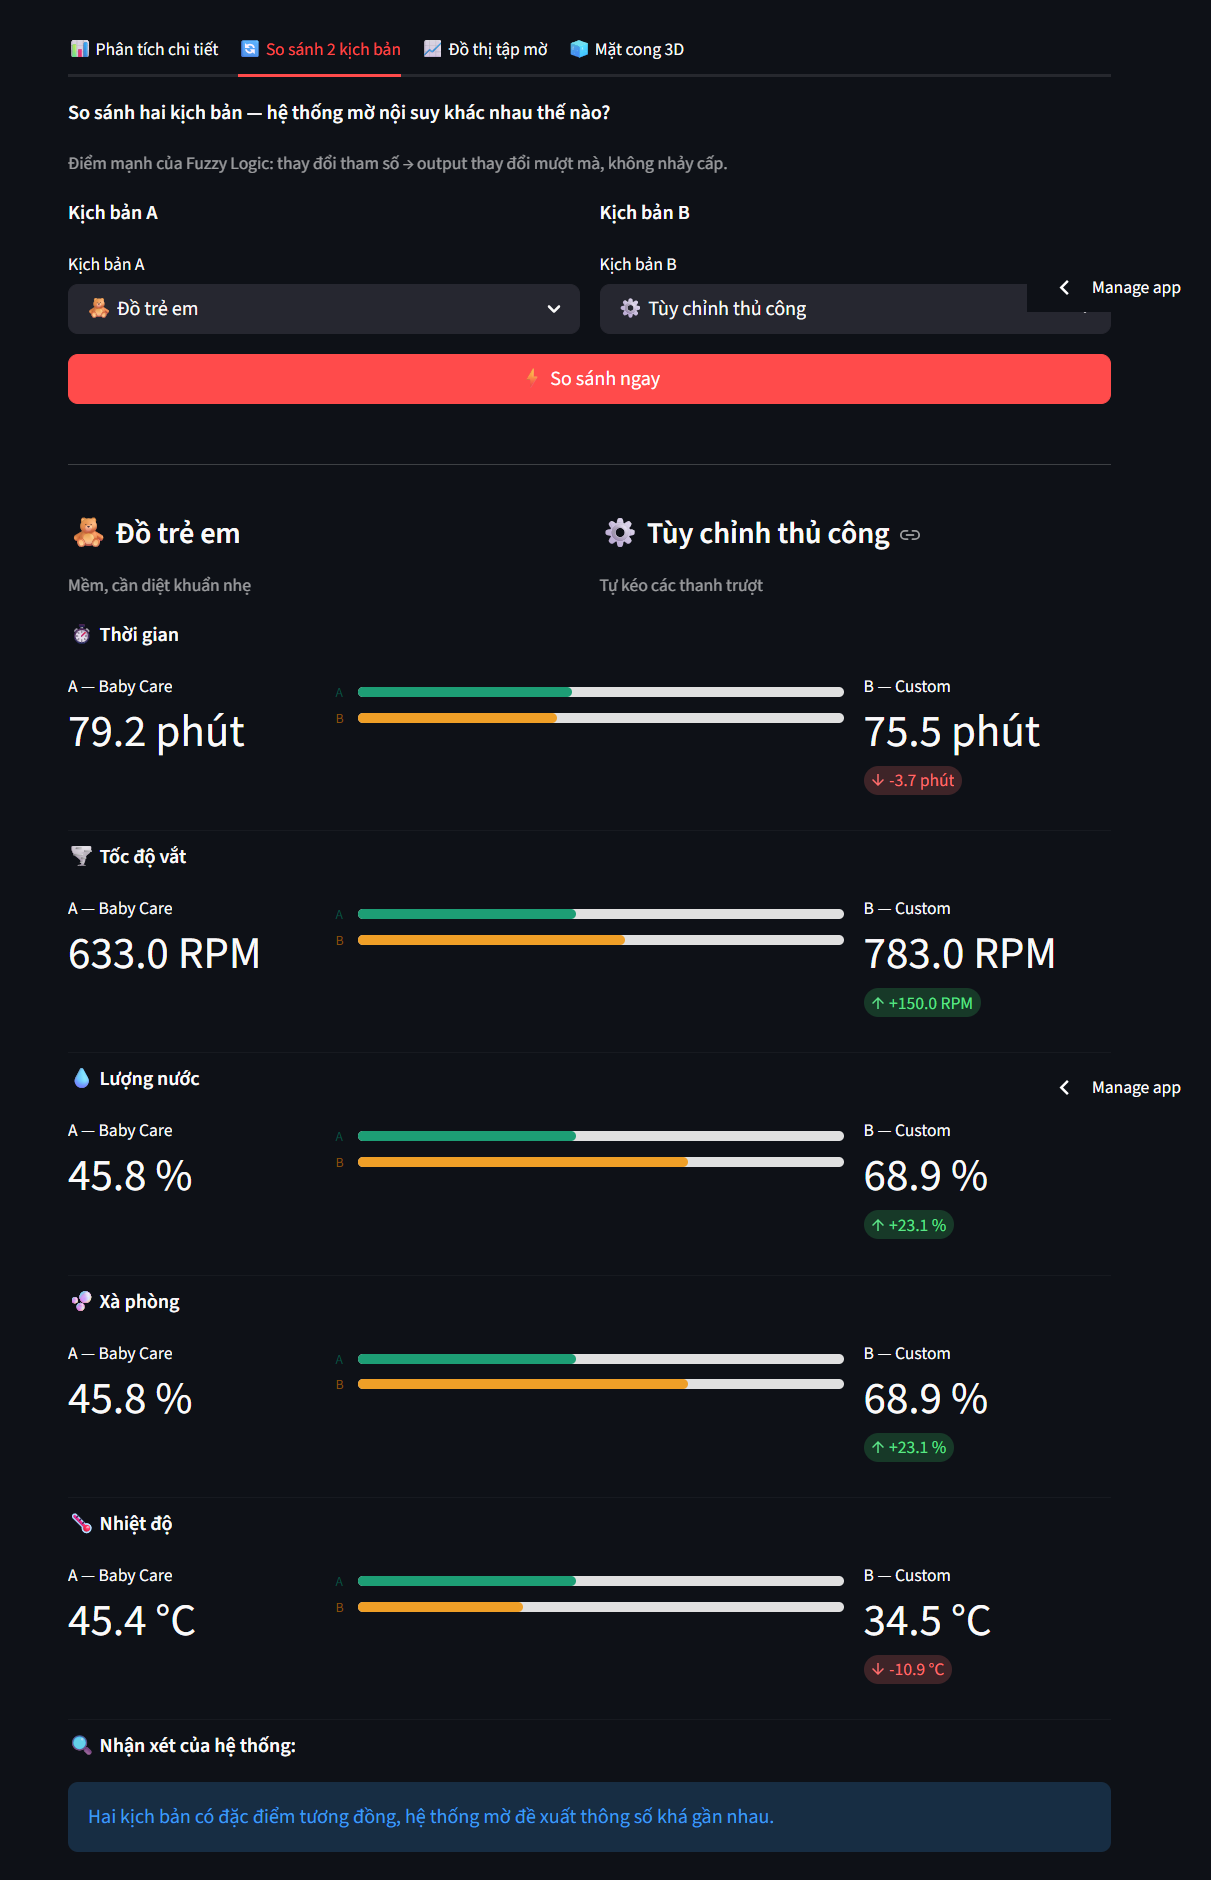
\includegraphics[width=0.9\textwidth]{images/tab_sosanh.png} 
    \caption{Trực quan hóa sự chênh lệch thông số giữa hai kịch bản giặt}
    \label{fig:tab_sosanh}
\end{figure}

\textbf{3. Tab Đồ thị tập mờ:} \\
Cho phép quan sát cơ chế nội suy của hệ suy diễn Mamdani. 5 đồ thị được bố cục dạng lưới $3+2$. Trên mỗi đồ thị, đường cong hàm liên thuộc được vẽ theo màu phân biệt, vùng tô màu biểu thị phần diện tích bị cắt ngọn sau khi áp dụng cường độ kích hoạt $\alpha$. Đường thẳng đứng màu đen đánh dấu tọa độ Trọng tâm $z^*$ — giá trị giải mờ thực tế.

\begin{figure}[H]
    \centering
    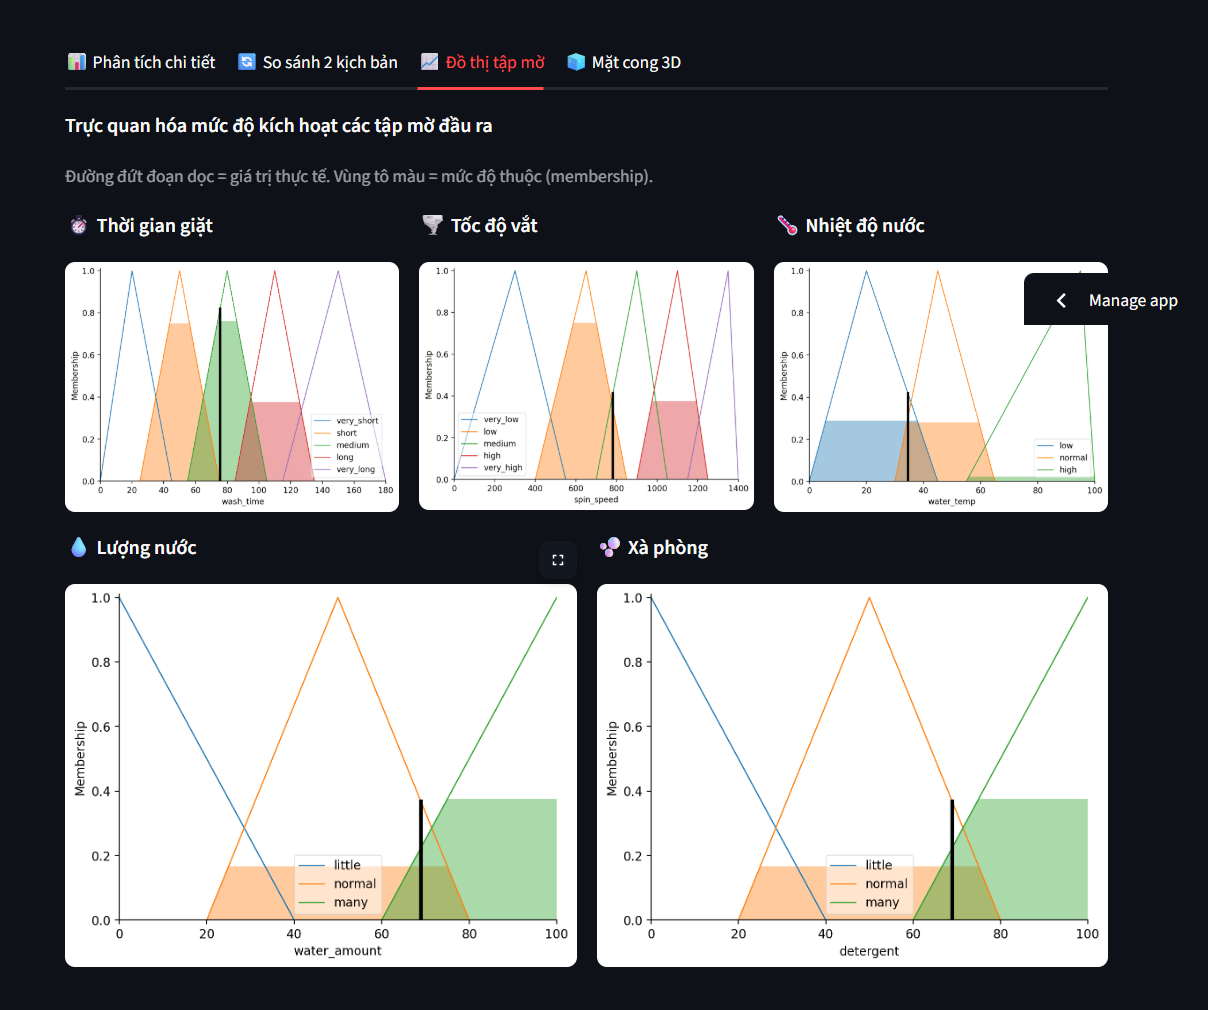
\includegraphics[width=0.95\textwidth]{images/tab_dothi.png} 
    \caption{Giao diện Tab Đồ thị tập mờ — Trực quan hóa mức độ kích hoạt và trọng tâm giải mờ (COA) của 5 biến đầu ra}
    \label{fig:tab_dothi}
\end{figure}

\textbf{4. Tab Mặt cong 3D:} \\
Minh chứng cho sự toàn vẹn của ma trận luật mờ. Mặt cong được tính toán bằng cách quét lưới $50 \times 50$ điểm (tổng cộng 2.500 lần tính toán), cố định biến Khối lượng và Độ bẩn theo kịch bản, đồng thời cho Độ nhạy vải (trục X) và Mức dầu mỡ (trục Y) chạy trên toàn bộ không gian nền. Điểm neo màu đỏ biểu thị tọa độ vận hành hiện tại.

\begin{figure}[H]
    \centering
    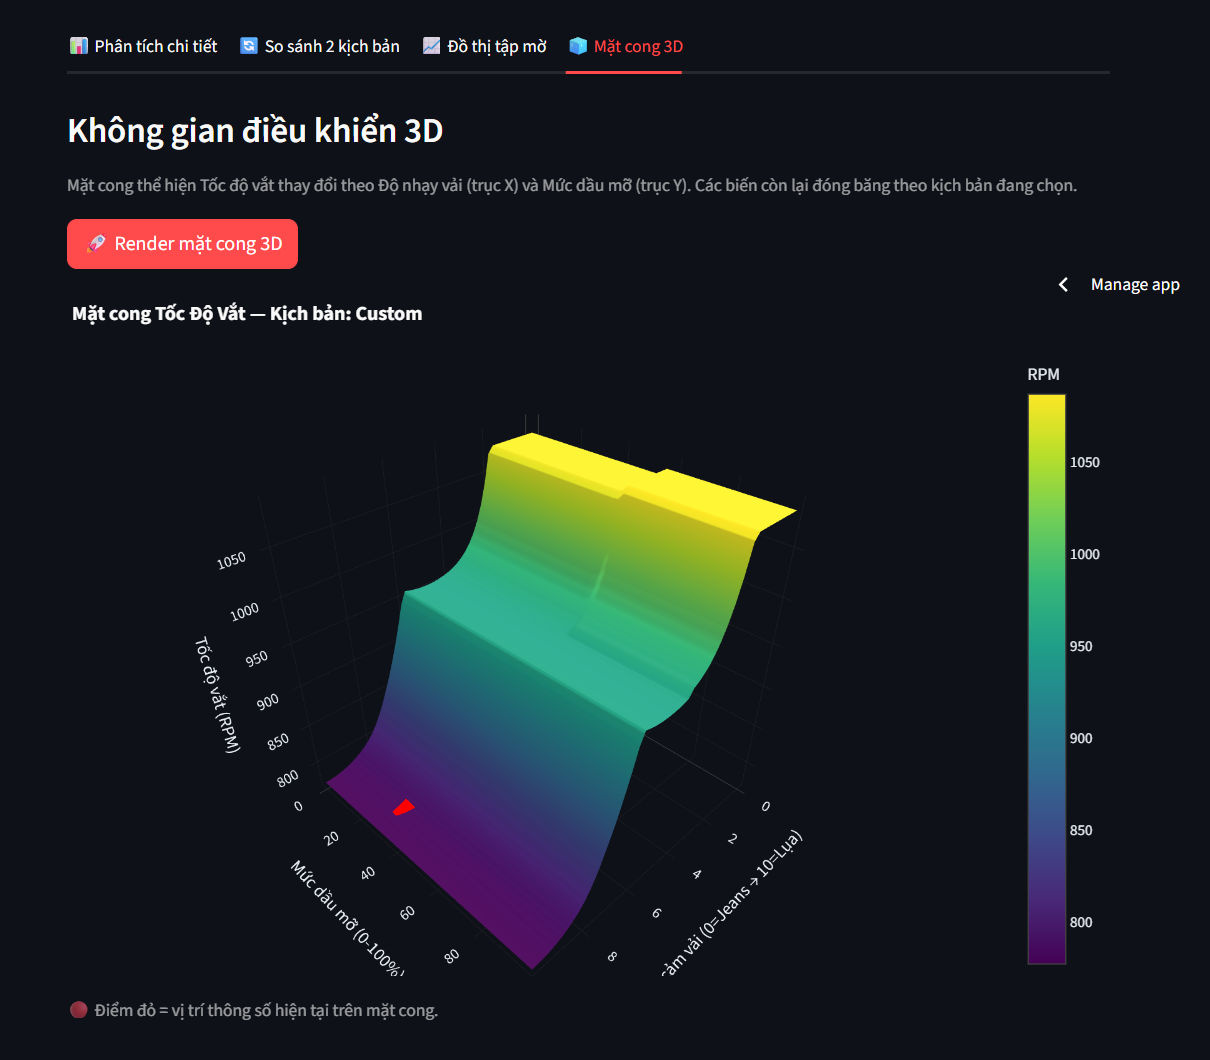
\includegraphics[width=0.85\textwidth]{images/tab_3d.png} 
    \caption{Tab Mặt cong không gian điều khiển 3D tương tác của tốc độ vắt}
    \label{fig:tab_3d}
\end{figure}

\subsection{Kết quả kiểm thử qua các kịch bản thực tế}
Để đánh giá độ tin cậy của thuật toán, hệ thống được đưa vào kiểm thử với 4 kịch bản. Các kịch bản này được nhóm nghiên cứu thiết lập mô phỏng lại những thói quen giặt giũ phổ biến trong thực tế hộ gia đình, bao phủ từ tải nhẹ đến tải nặng. Đặc biệt, một kịch bản "Trạng thái biên" được cố ý đặt tại đúng ranh giới giao cắt của các tập mờ nhằm kiểm chứng khả năng tính toán của hệ thống. Bảng \ref{tab:test_cases} trình bày đối chiếu thông số đầu ra giữa các kịch bản này.

\begin{table}[H]
    \centering
    \caption{Kết quả nội suy từ bộ điều khiển mờ cho các kịch bản kiểm thử}
    \label{tab:test_cases}
    \resizebox{\textwidth}{!}{
    \renewcommand{\arraystretch}{1.3}
    \begin{tabular}{|l|c|c|c|c|c|}
        \hline
        \textbf{Thông số} & \textbf{TC1: Heavy Duty} & \textbf{TC2: Delicates} & \textbf{TC3: Mixed Fabric} & \textbf{TC4: Baby Care} & \textbf{TC5: Duvet} \\
        \hline
        \multicolumn{6}{|c|}{\cellcolor[gray]{0.9}\textit{Biến đầu vào (Giả lập Cảm biến)}} \\
        \hline
        Khối lượng (kg) & $8.5$ & $1.5$ & $5.0$ & $3.5$ & $9.0$ \\
        Độ bẩn (\%)     & $95$  & $20$  & $50$  & $85$  & $40$  \\
        Dầu mỡ (\%)     & $90$  & $10$  & $50$  & $30$  & $15$  \\
        Nhạy cảm (Điểm) & $1$   & $9$   & $5$   & $8$   & $4$   \\
        \hline
        \multicolumn{6}{|c|}{\cellcolor[gray]{0.9}\textit{Biến đầu ra (Giá trị giải mờ COA thực tế)}} \\
        \hline
        Thời gian (phút)    & $130.6$ & $38.1$ & $80.0$ & $82.5$ & $91.7$ \\
        Tốc độ vắt (RPM)    & $1165$  & $452$  & $883$  & $631$  & $986$ \\
        Nhiệt độ ($^\circ$C)& $82.9$  & $21.7$ & $46.7$ & $45.4$ & $32.0$ \\
        Lượng nước (\%)     & $85.3$  & $14.7$ & $50.0$ & $45.8$ & $86.0$ \\
        Xà phòng (\%)       & $86.1$  & $14.7$ & $50.0$ & $45.8$ & $65.0$ \\
        \hline
    \end{tabular}
    }
\end{table}

\textbf{Đánh giá và Đối chiếu Baseline (Logic Boolean):} \\
Các kết quả tại Bảng \ref{tab:test_cases} chứng minh ma trận luật hoạt động vô cùng chuẩn xác (như kịch bản "TC2: Delicates" đã kích hoạt thành công \textit{Luật ghi đè} để ép tốc độ vắt xuống còn $452$ RPM bảo vệ vải lụa).

Đặc biệt, ưu thế nội suy của Logic mờ thể hiện rõ nhất tại kịch bản "TC3: Mixed Fabric" ($5.0$ kg đồ, $50\%$ bùn đất). Nếu sử dụng logic ngưỡng cứng phổ biến trên máy giặt truyền thống: ngưỡng khối lượng $\ge 5$ kg có thể lập tức kích hoạt mức nước trần $80\%$, và độ bẩn $\ge 50\%$ sẽ chốt cứng chu trình giặt ở $120$ phút. Nghĩa là tại trạng thái lấp lửng này, máy giặt Boolean rất dễ bị nhảy vọt lên mức tiêu thụ cao. 

Trong khi đó, bộ điều khiển Fuzzy đã tính toán ra diện tích chồng lấn và xuất ra một kết quả trung gian vô cùng mềm mại: Thời gian $80.0$ phút và Lượng nước $50.0\%$. Sự khác biệt này là minh chứng bằng số liệu cho khả năng tiết kiệm tài nguyên vượt trội và triệt tiêu hoàn toàn hiện tượng nhảy bậc của hệ thống nội suy mờ.

\subsection{Phân tích không gian điều khiển 3D}
Sức mạnh của Logic mờ không nằm ở các điểm rời rạc mà nằm ở tính liên tục của không gian nội suy. Bằng cách đóng băng 2 biến (Khối lượng và Độ bẩn) theo kịch bản và cho 2 biến còn lại (Độ nhạy vải, Mức dầu mỡ) quét qua toàn bộ không gian nền bằng lưới $50 \times 50$ điểm (tổng cộng 2.500 lần tính toán), hệ thống đã kết xuất thành công mặt cong 3D cho tín hiệu "Tốc độ vắt".

\begin{figure}[H]
    \centering
    \begin{subfigure}[b]{0.48\textwidth}
        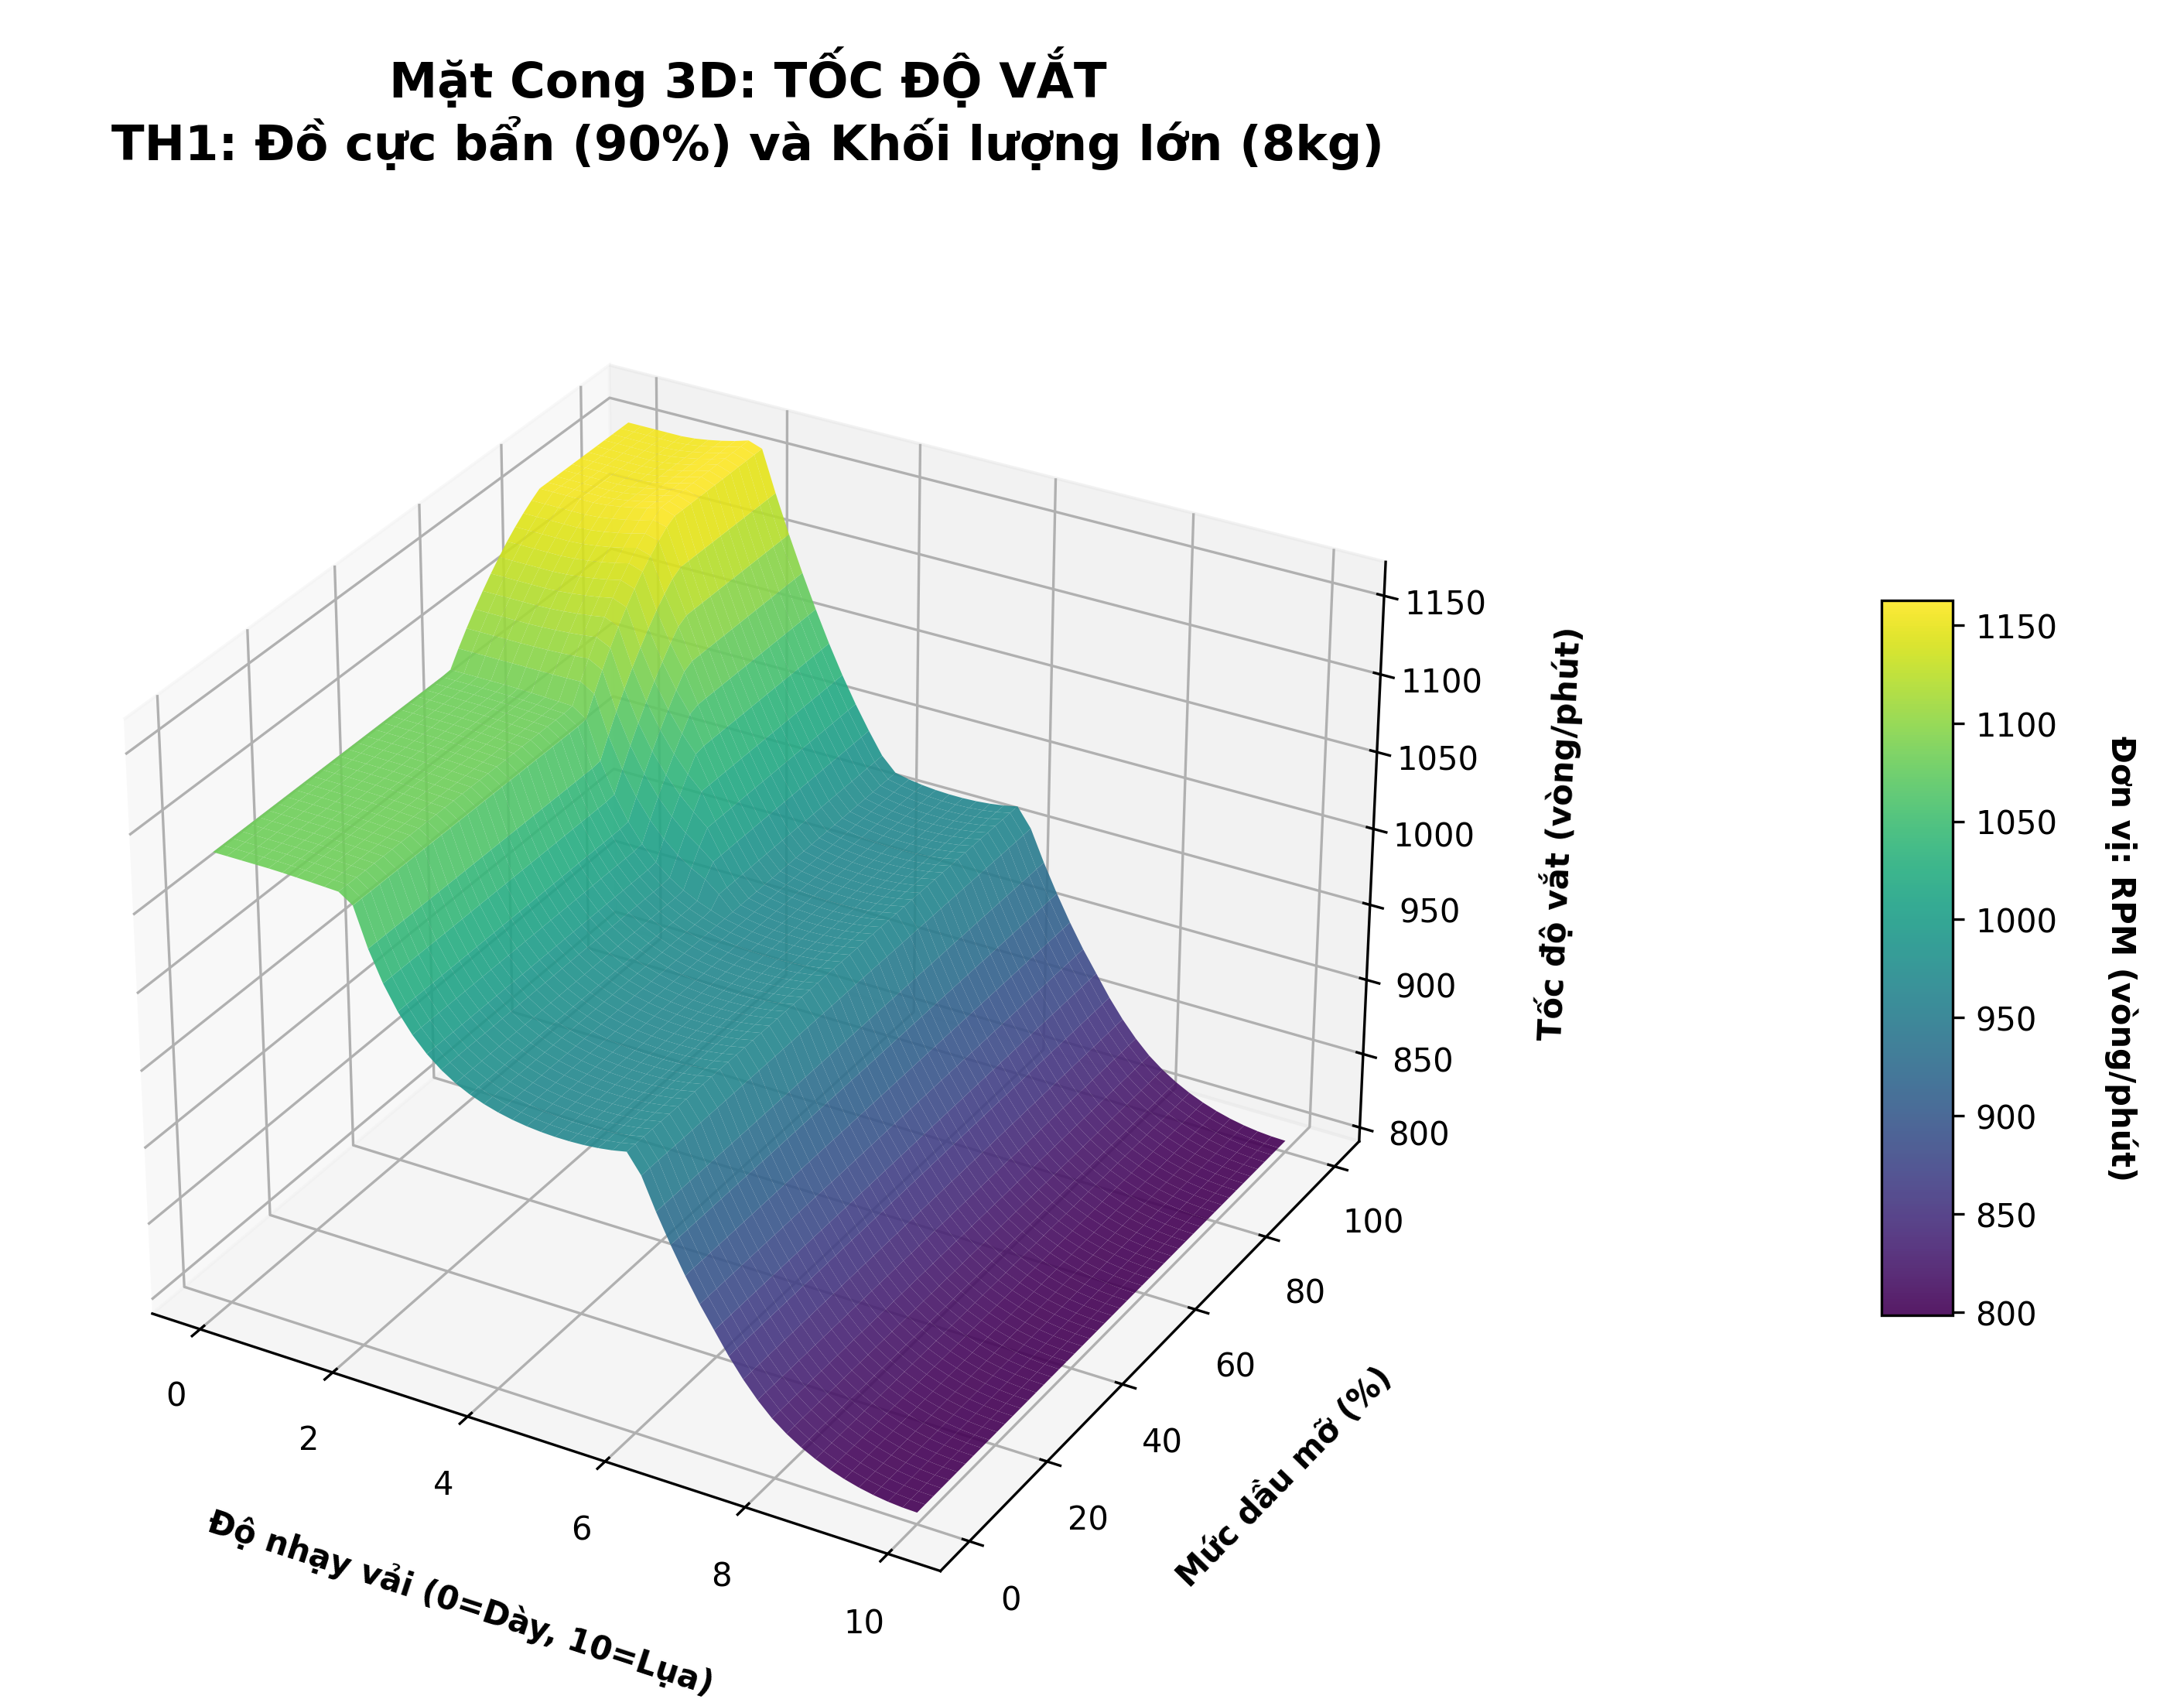
\includegraphics[width=\textwidth]{images/3d_spin_heavy_duty.png}
        \caption{Kịch bản Đồ bảo hộ (Tải nặng, cực bẩn)}
        \label{fig:3d_heavy}
    \end{subfigure}
    \hfill
    \begin{subfigure}[b]{0.48\textwidth}
        
\includegraphics[width=\textwidth]{images/3d_spin_delicates.png}
        \caption{Kịch bản Vải mỏng (Tải nhẹ, ít bẩn)}
        \label{fig:3d_delicate}
    \end{subfigure}
    \caption{Đối chiếu mặt cong không gian điều khiển Tốc độ vắt giữa hai tình huống thực tế}
    \label{fig:3d_surfaces}
\end{figure}

Sự khác biệt về cao độ giữa Hình \ref{fig:3d_heavy} và Hình \ref{fig:3d_delicate} chứng minh sự can thiệp hiệu quả của cấu trúc luật phân tầng. Ở kịch bản Đồ bảo hộ, mặt cong duy trì trần vận tốc rất cao để vắt kiệt nước, nhưng lập tức đổ dốc (hạ vòng quay) khi trục hoành tiến về vùng có sợi vải nhạy cảm. Ngược lại, ở kịch bản Vải mỏng, toàn bộ mặt cong bị ép phẳng ở mức tốc độ thấp để bảo vệ sợi lụa, bất chấp việc lượng dầu mỡ có tăng lên. Cuối cùng, sự trơn nhẵn của cả hai mặt cong khẳng định ma trận luật đã được thiết kế chuẩn xác, không tạo ra các lỗ hổng logic, đảm bảo động cơ hoạt động êm ái.

% ===================================================================
% CHƯƠNG 5: KẾT LUẬN VÀ HƯỚNG PHÁT TRIỂN
% ===================================================================
\section{Kết luận và Hướng phát triển}

\subsection{Kết quả đạt được}
Đối chiếu với các mục tiêu và câu hỏi nghiên cứu đã đặt ra tại Chương 1, đồ án đã hoàn thiện trọn vẹn các yêu cầu khoa học và kỹ thuật:
\begin{itemize}
    \item \textbf{Đối với RQ1:} Đề tài đã xây dựng thành công mô hình toán học lượng hóa các tín hiệu vật lý liên tục thành không gian 9 biến ngôn ngữ. Việc áp dụng hàm liên thuộc được căn chỉnh sát với giới hạn cơ khí của nguyên mẫu LG AI DD, đảm bảo tính khả thi khi áp dụng vào thực tiễn.
    \item \textbf{Đối với RQ2:} Bài toán xung đột mục tiêu (giữa hiệu năng làm sạch và tiết kiệm tài nguyên) được giải quyết hiệu quả thông qua kiến trúc luật phân tầng 3 lớp. Cơ sở tri thức gồm 19 luật mờ đã thể hiện được sự mềm dẻo, đặc biệt là sự can thiệp kịp thời của các luật ghi đè an toàn nhằm bảo vệ tối đa cấu trúc sợi vải.
    \item \textbf{Đối với RQ3:} Năng lực đáp ứng và tính ổn định của hệ suy diễn Mamdani được minh chứng trực quan qua bề mặt trơn nhẵn của không gian điều khiển 3D. Tại các kịch bản có trạng thái giao thoa cận biên, thuật toán giải mờ Trọng tâm cho thấy khả năng nội suy liên tục xuất sắc, hoàn toàn triệt tiêu hiện tượng nhảy bậc thường thấy ở logic Boolean.
\end{itemize}
Bên cạnh các giá trị lý thuyết, đồ án cũng đã đóng gói thành công bộ thuật toán thành một ứng dụng web trực quan, cho phép mô phỏng và kiểm chứng thời gian thực toàn bộ chu trình giải mờ.

\subsection{Hạn chế của mô hình}
Dưới góc độ lý thuyết điều khiển tự động, hệ thống hiện tại tồn tại hai nhược điểm cốt lõi:
\begin{itemize}
    \item \textbf{Cơ chế điều khiển vòng hở:} Đây là hạn chế lớn nhất của hệ thống. Bộ điều khiển hiện tại chỉ tiến hành lấy mẫu dữ liệu từ cảm biến một lần duy nhất lúc khởi động. Sự thiếu vắng của vòng lặp phản hồi khiến máy giặt không thể tự nhận biết và hiệu chỉnh nếu độ đục của nước thay đổi ngoài dự kiến trong lúc đang giặt.
    \item \textbf{Đặc tính hình học tuyến tính từng khúc:} Việc sử dụng hoàn toàn hàm tam giác giúp tối ưu chi phí phần cứng nhưng làm mất đi tính khả vi tại các điểm chuyển mạch. Do đó, sự biến thiên trên mặt cong 3D ở một số cực trị chưa đạt được độ trơn nhẵn tuyệt đối như khi áp dụng hàm phi tuyến.
\end{itemize}

\subsection{Hướng phát triển tương lai}
\begin{itemize}
    \item \textbf{Tích hợp hệ thống ANFIS:} Nâng cấp bộ điều khiển bằng mạng nơ-ron thích nghi. Thuật toán học máy sẽ tự động phân tích dữ liệu lịch sử giặt giũ của gia đình để tự tinh chỉnh và xê dịch tọa độ $(a, b, c)$ của các hàm liên thuộc, giải quyết triệt để sự phụ thuộc vào ý chí chủ quan của người lập trình.
    \item \textbf{Nâng cấp điều khiển vòng kín:} Triển khai mô hình lên các vi điều khiển nhúng (STM32/ESP32). Thiết bị sẽ liên tục ping dữ liệu độ đục nước mỗi 5 phút để thuật toán đánh giá lại mệnh đề kết luận, linh hoạt ngắt chu trình sớm nhằm tiết kiệm điện nước.
    \item \textbf{Hoàn thiện hệ sinh thái IoT:} Mở rộng thêm đầu vào là nhiệt độ và độ cứng của nước tại địa phương để nội suy tỷ lệ hóa chất. Đồng thời tích hợp giao thức truyền tin MQTT để đẩy các báo cáo phân tích sinh thái (tiêu thụ điện/nước) trực tiếp về smartphone của người dùng.
\end{itemize}

% ===================================================================
% TÀI LIỆU THAM KHẢO
% ===================================================================
\newpage
\renewcommand{\refname}{Tài liệu tham khảo}
\begin{thebibliography}{9}
\addcontentsline{toc}{section}{Tài liệu tham khảo}

\bibitem{zadeh1965} 
Zadeh, L. A. (1965). Fuzzy sets. \textit{Information and Control}, 8(3), 338–353.

\bibitem{mamdani1975} 
Mamdani, E. H., \& Assilian, S. (1975). An experiment in linguistic synthesis with a fuzzy logic controller. \textit{International Journal of Man-Machine Studies}, 7(1), 1–13.

\bibitem{skfuzzy} 
Warner, J., et al. (2019). \textit{scikit-fuzzy: A fuzzy logic toolkit for SciPy}. URL: \url{https://pythonhosted.org/scikit-fuzzy/}

\bibitem{lg_specs} 
LG Electronics. (2021). \textit{LG AI DD Inverter 10kg (FV1410S3B) Specifications \& User Manual}. URL: \url{https://www.lg.com/}

\end{thebibliography}

\newpage
\appendix
\section{Phụ lục: Ma trận cơ sở tri thức (19 Luật Mờ)}
Bảng dưới đây liệt kê đầy đủ 19 quy luật điều khiển cốt lõi sau khi đã áp dụng kỹ thuật cắt tỉa (\textit{Rule Pruning}). Các luật này được trích xuất trực tiếp từ mã nguồn thực thi (\textit{fuzzy\_washing.py}), định hình toàn bộ luồng suy diễn của hệ thống.

\begin{table}[H]
    \centering
    \caption{Chi tiết 19 quy luật mờ IF-THEN của bộ điều khiển (Ánh xạ từ Source Code)}
    \label{tab:full_rules}
    \resizebox{\textwidth}{!}{
    \renewcommand{\arraystretch}{1.3}
    \begin{tabular}{|c|p{7cm}|p{8cm}|}
        \hline
        \textbf{Luật} & \textbf{Mệnh đề Điều kiện (IF)} & \textbf{Mệnh đề Kết luận (THEN)} \\
        \hline
        \multicolumn{3}{|c|}{\cellcolor[gray]{0.9}\textbf{Nhóm luật Kịch bản Toàn diện}} \\
        \hline
        Rule 1 & Độ bẩn(Nhiều) AND Mỡ(Nhiều) AND Vải(Ít nhạy cảm) AND Khối lượng(Nhiều) & Thời gian(Rất dài), Vắt(Rất cao), Nước(Nhiều), Xà phòng(Nhiều), Nhiệt độ(Cao) \\
        \hline
        Rule 2 & Độ bẩn(Ít) AND Mỡ(Không) AND Vải(Rất nhạy cảm) AND Khối lượng(Ít) & Thời gian(Rất ngắn), Vắt(Rất thấp), Nước(Ít), Xà phòng(Ít), Nhiệt độ(Thấp) \\
        \hline
        Rule 3 & Độ bẩn(Vừa) AND Mỡ(Hỗn hợp) AND Vải(Bình thường) AND Khối lượng(Vừa) & Thời gian(Vừa), Vắt(Vừa), Nước(Bình thường), Xà phòng(Bình thường), Nhiệt độ(Vừa) \\
        \hline
        Rule 4 & Độ bẩn(Nhiều) AND Mỡ(Hỗn hợp) AND Vải(Rất nhạy cảm) & Thời gian(Dài), Vắt(Thấp), Xà phòng(Bình thường), Nhiệt độ(Cao) \\
        \hline
        Rule 5 & Độ bẩn(Vừa) AND Mỡ(Không) AND Vải(Bình thường) AND Khối lượng(Nhiều) & Thời gian(Dài), Vắt(Cao), Nước(Nhiều), Xà phòng(Bình thường), Nhiệt độ(Vừa) \\
        \hline
        \multicolumn{3}{|c|}{\cellcolor[gray]{0.9}\textbf{Nhóm luật Bổ trợ Tài nguyên \& Đơn lẻ}} \\
        \hline
        Rule 6 & Khối lượng(Ít) & Lượng nước(Ít), Xà phòng(Ít) \\
        \hline
        Rule 7 & Khối lượng(Nhiều) & Lượng nước(Nhiều), Xà phòng(Nhiều) \\
        \hline
        Rule 8 & Mỡ(Nhiều) & Xà phòng(Nhiều), Nhiệt độ(Cao) \\
        \hline
        Rule 9 & Vải(Rất nhạy cảm) & Thời gian(Ngắn), Tốc độ vắt(Thấp) \\
        \hline
        Rule 10 & Vải(Ít nhạy cảm) AND Độ bẩn(Nhiều) & Thời gian(Dài), Tốc độ vắt(Cao) \\
        \hline
        Rule 11 & Độ bẩn(Ít) & Thời gian(Ngắn) \\
        \hline
        Rule 12 & Độ bẩn(Vừa) & Thời gian(Vừa) \\
        \hline
        Rule 13 & Độ bẩn(Nhiều) & Thời gian(Dài) \\
        \hline
        Rule 14 & Mỡ(Không) & Nhiệt độ(Thấp) \\
        \hline
        Rule 15 & Mỡ(Hỗn hợp) & Nhiệt độ(Vừa) \\
        \hline
        Rule 16 & Khối lượng(Vừa) & Lượng nước(Bình thường), Xà phòng(Bình thường) \\
        \hline
        Rule 17 & Vải(Bình thường) & Tốc độ vắt(Vừa) \\
        \hline
        Rule 18 & Khối lượng(Nhiều) & Thời gian(Dài), Tốc độ vắt(Cao) \\
        \hline
        Rule 19 & Khối lượng(Ít) & Thời gian(Ngắn), Tốc độ vắt(Thấp) \\
        \hline
    \end{tabular}
    }
\end{table}

\end{document}